\documentclass{llncs}
\usepackage{enumerate}% http://ctan.org/pkg/enumerate
\usepackage{multirow}
\usepackage{amsmath,amssymb}
\usepackage{url}
\usepackage{overpic}
\usepackage{enumerate}
\usepackage{graphicx}        % standard LaTeX graphics tool
\usepackage{tikz}        % standard LaTeX graphics tool
\usepackage{pgfplots}

%\usetikzlibrary{arrows}
%\usetikzlibrary{quotes,angles}
\usepackage{subfigure}                                 % authors: subfigures
\usepackage[ruled,vlined,linesnumbered]{algorithm2e}   % authors: last version of algorithm display
\usepackage{todonotes}

\usepackage{booktabs}


\newcommand{\ie}{\emph{i.e.} }
\newcommand{\eg}{\emph{e.g.} }
\newcommand{\wrt}{\emph{w.r.t.} }
\newcommand{\wnlog}{w.l.o.g. }
\newcommand{\Zr}{\ensuremath{\mathbb{Z}[\rho]}}
\newcommand{\C}{\ensuremath{\mathbb{C}}}
\newcommand{\E}{\ensuremath{\mathcal{E}}}

\definecolor{cgeometry}{RGB}{255, 120, 0}
\definecolor{clquatre}{RGB}{198,219,239}
\definecolor{cltrois}{RGB}{158,202,225}
\definecolor{cldeux}{RGB}{107,174,214}
\definecolor{clun}{RGB}{49,130,189}
\definecolor{clzero}{RGB}{8,81,156}

\title{Interactive Curvature Tensor Visualization on Digital
Surfaces\thanks{This work has been mainly funded by \textsc{DigitalSnow}
ANR-11-BS02-009, \textsc{KIDICO} ANR-2010-BLAN-0205 and \textsc{PRIMES Labex}
ANR-11-LABX-0063/ ANR-11-IDEX-0007 research grants.}}

\author{H\'el\`ene Perrier\inst{1}\and J\'er\'emy Levallois\inst{1,2}\and David
Coeurjolly\inst{1}\and Jean-Philippe Farrugia\inst{1}\and Jean-Claude
Iehl\inst{1}\and Jacques-Olivier Lachaud\inst{2} }

%\address[liris]{Universit\'e de Lyon, CNRS, INSA-Lyon, LIRIS, UMR5205, F-69621, France}
%\address[lama]{Universit\'e de Savoie, CNRS, LAMA, UMR 5127, F-73776, France}

 \institute{ Universit\'e de Lyon, CNRS\\
   LIRIS, UMR5205, F-69621, France
%   \email{\{david.coeurjolly,jeremy.levallois\}@liris.cnrs.fr}
   \and
Universit\'e de Savoie, CNRS\\
LAMA, UMR5127, F-73776, France\\
%\email{jacques-olivier.lachaud@univ-savoie.fr}
}

\graphicspath{{./figs/}}
%fonts bonanza
\usepackage{amsmath,amssymb,amsfonts}
\usepackage{pifont}% http://ctan.org/pkg/pifont
\newcommand{\CheckMark}{\ding{51}}%
\newcommand{\CrossMark}{\ding{55}}%
% Zapf font
\usepackage[mathscr]{euscript}
\DeclareFontFamily{OT1}{pzc}{}
\DeclareFontShape{OT1}{pzc}{m}{it}%
              {<-> s * [1.2] pzcmi7t}{}
\DeclareMathAlphabet{\mathpzc}{OT1}{pzc}{m}{it}
% rescaling cal to be a touch smaller
\DeclareFontFamily{OMS}{fcmsy}{\skewchar\font48 }
\DeclareFontShape{OMS}{fcmsy}{m}{n}{%
         <-5.5> [.96] cmsy5     <5.5-6.5> [.96] cmsy6
      <6.5-7.5> [.96] cmsy7     <7.5-8.5> [.96] cmsy8
      <8.5-9.5> [.96] cmsy9     <9.5->  [.96] cmsy10
      }{}
\DeclareFontShape{OMS}{fcmsy}{b}{n}{%
       <-6> [.96] cmbsy5
      <6-8> [.96] cmbsy7
      <8->  [.96] cmbsy10
      }{}
\DeclareMathAlphabet{\mathcal}{OMS}{fcmsy}{m}{n}
%\usepackage{bbm}

\usepackage{mathtools}% http://ctan.org/pkg/mathtools
\usepackage{calc}% http://ctan.org/pkg/calc

\newcommand*{\mytilde}[2][0pt]{%
  \setbox0=\hbox{$#2$}%
  \tilde{\mathrlap{\phantom{\rule{\wd0}{\ht0+{#1}}}}\smash{#2}}%
}
\newcommand*{\mywidetilde}[2][0pt]{%
  \setbox0=\hbox{$#2$}%
  \widetilde{\mathrlap{\phantom{\rule{\wd0}{\ht0+{#1}}}}\smash{#2}}%
}

\newtheorem{Definition}{Definition}
\newtheorem{Theorem}{Theorem}
\newtheorem{Proposition}{Proposition}
\newtheorem{Corollary}{Corollary}
\newtheorem{Problem}{Problem}
\newtheorem{Lemma}{Lemma}
\newtheorem{Claim}{Claim}

%%Space, Lattices
\newcommand{\Z}{{\mathbb{Z}}}
\newcommand{\N}{{\mathbb{N}}}
\newcommand{\R}{{\mathbb{R}}}
\newcommand{\M}{\mathcal{M}}
\newcommand{\B}{\mathcal{B}_R}

\newcommand{\BT}[1]{\ensuremath{\partial #1}}
\newcommand{\Bd}[1]{\ensuremath{\partial #1}}
\newcommand{\dS}{\BT X}
\newcommand{\Body}[2]{\ensuremath{\lbrack #1 \rbrack_{#2}}}

\newcommand{\Shape}{\ensuremath{X}}
\newcommand{\DigShape}{\ensuremath{Z}}
\newcommand{\Boundary}[1]{\ensuremath{\partial #1}}
\newcommand{\DigBoundary}[1]{\ensuremath{Bd(#1)}}
\newcommand{\Shapes}{\ensuremath{\mathbb{X}}}
\newcommand{\vx}{\ensuremath{\mathbf{x}}}
\newcommand{\vxH}{\ensuremath{\hat{\mathbf{x}}}}
\newcommand{\vp}{\ensuremath{\mathbf{p}}}
\newcommand{\vw}{\ensuremath{\mathbf{w}}}
\newcommand{\vn}{\ensuremath{\mathbf{n}}}
\newcommand{\Dig}{\ensuremath{\mathtt{G}}}
\newcommand{\DigF}[2]{\ensuremath{\Dig_{#2}\left(#1\right)}}
\newcommand{\DSh}{\DigF{\Shape}{h}}

\newcommand{\MCard}{\ensuremath{\mathrm{Card}}}
\newcommand{\Area}{\ensuremath{\mathrm{Area}}}
\newcommand{\Vol}{\ensuremath{\mathrm{Vol}}}
\newcommand{\AreaC}[0]{\ensuremath{\widehat{\Area}}}
\newcommand{\VolC}[0]{\ensuremath{\widehat{\Vol}}}
\newcommand{\Ball}[2]{\ensuremath{B_{#1}\left(#2\right)}}

%% Curvature notations
\newcommand{\Curv}{\ensuremath{\kappa}}
\newcommand{\MeanCurv}{\ensuremath{H}}
\newcommand{\GaussCurv}{\ensuremath{K}}
\newcommand{\PrincCurv}[1]{\ensuremath{\kappa_{#1}}}
\newcommand{\PrincDir}[1]{\ensuremath{\vw_{#1}}}
\newcommand{\NormalDir}{\ensuremath{\vn}}

%% Pottmann curvature estimators
\newcommand{\CurvT}[1]{\ensuremath{\tilde{\Curv}^{#1}}}
\newcommand{\MeanCurvT}[1]{\ensuremath{\tilde{\MeanCurv}^{#1}}}
\newcommand{\GaussCurvT}[1]{\ensuremath{\tilde{\GaussCurv}^{#1}}}
\newcommand{\PrincCurvT}[2]{\ensuremath{\tilde{\PrincCurv{}}_{#1}^{#2}}}
\newcommand{\PrincDirT}[2]{\ensuremath{\tilde{\PrincDir{}}_{#1}^{#2}}}
\newcommand{\NormalDirT}[1]{\ensuremath{\tilde{\NormalDir{}}^{#1}}}

%% II curvature estimators
\newcommand{\CurvH}[1]{\ensuremath{\hat{\Curv}^{#1}}}
\newcommand{\MeanCurvH}[1]{\ensuremath{\hat{\MeanCurv}^{#1}}}
\newcommand{\GaussCurvH}[1]{\ensuremath{\hat{\GaussCurv}^{#1}}}
\newcommand{\PrincCurvH}[2]{\ensuremath{\hat{\PrincCurv{}}_{#1}^{#2}}}
\newcommand{\PrincDirH}[2]{\ensuremath{\hat{\PrincDir{}}_{#1}^{#2}}}
\newcommand{\NormalDirH}[1]{\ensuremath{\hat{\NormalDir{}}^{#1}}}

%%Formulas
\newcommand{\EqDef}{\!\ensuremath{\mathrel{\mathop:}=}\!}
%\newcommand{\EqDef}{\smash{\ensuremath{\stackrel{\text{def}}{=}}}}

%% Misc.
\newcommand{\txtblue}[1]{\textcolor{blue}{ #1}}
\newcommand{\txtgreen}[1]{\textcolor{green}{ #1}}
\newcommand{\txtred}[1]{\textcolor{red}{ #1}}


\DeclareMathOperator*{\argmin}{arg\,min}

\begin{document}
\maketitle


\begin{abstract}\sloppy
  Interactive visualization is a very convenient tool to explore
  complex scientific data or to explore different parameter settings
  for a given processing algorithm. In this article, we present a tool
  to efficiently explore the curvature tensor on the boundary of
  potentially large and dynamic digital objects (mean and gaussian curvature,
  principal curvatures, principal directions and normal vector
  field). More precisely, we combine a fully parallel pipeline on GPU
  to extract an adaptive triangulated isosurface of the digital
  object, with a curvature tensor estimation at each surface point
  based on integral invariants. Integral invariants being parametrized
  by a given ball radius, our proposal allows us to explore
  interactively different radii and thus select the appropriate scale
  to which the computation is performed and visualized.

\keywords{Isosurface Visualization, Digital Geometry, Curvature
  Estimation, GPU.}
\end{abstract}

\section{Introduction}
\label{sec:introduction}

Volumetric objects are being more and more popular in many
applications ranging from object modeling and rendering in Computer
Graphics to geometry processing in Medical Imaging or Material
Sciences. When considering large volumetric data, interactive
%visualization of such images (or isovalue surfaces) is a complex
visualization of those objects (or isosurfaces) is a complex
problem. Such issues become even more difficult when dynamic
%volumetric datasets are considered. Beside such isosurface
volumetric datasets are considered. Beside
visualization, we are also interested in performing geometry
processing on the digital object and to explore different parameter
settings of the geometry processing tool.  In this work, we focus on
interactive visualization of volumetric data isosurfaces combined with
a curvature tensor (mean/Gaussian curvature, principal curvatures
directions, \ldots) estimation at each point of the digital
surface.
%Curvature maps on a given isosurface are key information when
%exploring 3D structures in Material Sciences \todo{REF}.
Furthermore,
most curvature estimators require a parameter fixing the scale
to which the computation is performed. For short, such parameter
(integration radius, convolution kernel size, \ldots) specifies noise
level on the object surface. As a consequence, exploring interactively
different values of such parameter is mandatory.
\vspace{0.2cm}

\noindent\textbf{Contributions}\quad In this work, we propose a framework to
perform interactive visualization of complex 3D digital structures combined with
a dynamic curvature tensor estimation. More precisely, we define a fully data
parallel process on GPU (Graphics Processor Unit) hardware to both efficiently
extract adaptive isosurface and compute per vertex curvature tensor using
Integral Invariants estimators. Hence, this system allows us to visualize
curvature tensor in real-time on large dynamic objects. Our approach combines a
GPU implementation of pointerless octrees to represent the data, an adaptive
viewpoint-dependent mesh extraction, and a GPU implementation of integral
invariant curvature estimators.


\vspace{0.2cm}

\sloppy\noindent\textbf{Related works}\quad Extracting and Visualizing
isosurface on volumetric data has been widely investigated since the
seminal Marching Cubes approach by \textsc{Lorensen} and
\textsc{Cline}~\cite{lorensen1987marching}. This approach being data parallel,
GPU implementation of this method is very efficient
\cite{tatarchuk2007real}. However, such technique generates a lot of
triangles which is not well suited to large digital data. Hence,
adaptive approaches have been proposed in order to optimize the
triangular mesh resolution to the object geometry or depending on the
viewpoint. In this topic, many solutions have been developed in
Computer
Graphics~\cite{shu1995adaptive,schaefer2004dual,lengyel2010voxel,DBLP:journals/cgf/LewinerMPPL10,DBLP:journals/cvgip/LobelloDD14}.
The method developed by \textsc{Lengyel} \textit{et al.}
\cite{lengyel2010voxel} is the best suited to our needs.
%However, it
%was only developed on CPU to visualize in real-time static or near
%static data, combining octree with new Marching Cubes configurations
%to generate adaptive meshes.
It combines an octree space partitioning with new Marching Cubes configuration
to generate adaptive meshes, but was only developed on the CPU to visualize
static or near static data.
In this paper we propose a full GPU pipeline
%inspired from this method.
inspired from this method, using a GPU-friendly Lod criterion to maintain a view dependent triangulation.
%It leaves the CPU free for other tasks and avoids synchronization with the GPU.
%Our high framerate also allows
Our high framerate allows
this method to run in real-time on fully dynamic data.
%The triangulation is controlled by a GPU LoD criterion
%that ensures that
%triangles project onto more than one pixel, thus removing geometrical
%aliasing.

Curvature estimation on discrete or digital surface has also been
widely investigated. In \cite{CVIU2014}, authors propose digital
versions of Integral Invariant estimators
\cite{Pottmann2007,Pottmann2009} in order to estimate the complete
curvature tensor (mean/Gaussian curvatures, principal curvatures,
principal curvature directions, normal vector field) on digital
surfaces. Such approaches are based on an integration principle using
a spherical kernel of a given radius. Additionally, authors have
demonstrated that these estimators have multigrid convergence
properties. In this article, we propose an efficient GPU
implementation of such estimators in order to visualize, in real-time,
such curvature maps and allowing us to interactively explore different
values of the spherical kernel radius.




\section{Curvature Tensor Estimation}
\label{sec:curv-tens-estim}

\sloppy In our context, we consider digital shapes (any subset $Z$ of $\Z^d$)
and boundaries of digital shapes $\DigBoundary{Z}$. We denote by $\DSh$ the
Gauss digitization of $\Shape$ in a $d-$dimensional grid with grid step $h$,
\emph{i.e.}  $\DSh \EqDef \{ \vz \in \Z^d,\, h\cdot\vz\in\Shape\}$. For such
digitized set $\DigShape\EqDef\DSh$, $\Body{\DigShape}{h}$ is a subset of $\R^d$
corresponding to the union of hypercubes centered at $h\cdot \vz$ for $\vz\in Z$
with edge length $h$. By doing so, both $\partial\Shape$ and
$\partial\Body{Z}{h}$ are topological boundary of objects lying in the same
space (See Fig. \ref{fig:notations}-b). Note that the combinatorial digital
boundary $\DigBoundary{Z}$ of $Z$ made of cells in a cellular Cartesian complex
(\emph{pointels}, \emph{linels}, \emph{surfels}, \ldots), can be trivially
embedded into $\R^d$ such that it coincides with $\partial\Body{Z}{h}$.


\begin{figure}[t]{\small
    \begin{center}
      \subfigure[]{\begin{overpic}[width=5cm]{figs/integral2D_2}
          \put(42,28){$\times$}
          \put(46,32){$\vx$}
          \put(55,45){$\Ball{R}{\vx}$}
          \put(1,10){$\dS$}
          \put(15,5){$\Shape$}
      \end{overpic}}~~~~~~
      \subfigure[]{\begin{overpic}[width=5cm]{figs/notation_2}
          \put(62,0.5){$h \cdot \vz \in \Shape \cap \Ball{R}{\vx}$}
          \put(55,45){$\Ball{R}{\vx}$}
          \put(42,28.5){$\times$}
          \put(45,32.5){$\vx$}
          \put(45,16.5){$h$}
          %\put(88,39){$\Proj(p)$}
          \put(1.5,10){$\partial \Shape$}
          \put(15,7){$\partial \Body{\DSh}{h}$}
      \end{overpic}}
      \vspace{-0.4cm}
    \end{center}}
    \caption{Integral invariant computation $(a)$ and
      notations $(b)$ in dimension 2 \cite{CVIU2014}.\label{fig:notations}}
\end{figure}

In \cite{DGCI2013}, authors have defined the 2D digital curvature estimator
$\CurvH{R}$ and the 3D digital mean curvature estimator $\MeanCurvH{R}$ based on
the digital volumetric integral $\VolC(Y,h) \EqDef h^d \MCard(Y)$ with
$\MCard(Y)$ the number of digital points of the intersection between a ball
$\Ball{R/h}{\vx/h}$ of digital radius $R/h$ and $\DigShape$ (we denote such
quantity $\AreaC(Y,h)$ in dimension 2):
%
\begin{Definition}
  %
  Given the Gauss digitization $Z\EqDef\DSh$ of a shape $\Shape \subset \R^2$
  (or $\R^3$ for the 3D mean curvature estimator), {\em digital curvature
  estimators} are defined for any point $\vx \in \R^2$ (or $\R^3$) as:
  %
  \begin{align}
    \forall 0 < h < R,\quad
    &\CurvH{R}(Z,\vx,h) \EqDef \frac{3\pi}{2R}
    - \frac{3\AreaC(\Ball{R/h}{\vx/h} \cap
    {Z}, h)}{R^3}\,,\label{eq:dig-curvature-estimator-k}\\
    &\MeanCurvH{R}(Z,\vx,h) \EqDef \frac{8}{3R}
    - \frac{4\VolC(\Ball{R/h}{\vx/h} \cap
    Z, h)}{\pi R^4}\,.\label{eq:dig-curvature-estimator-H}
  \end{align}
  %
  where $\Ball{R/h}{\vx/h}$ is the ball of digital radius $R/h$ centered on
  digital point $(\vx/h) \in Z$.
  %
  % \AreaC(\Ball{R/h}{\vx/h} \cap \Body{\DSh}{h}, h) \EqDef h^2 \MCard(
  % \Ball{R/h}{\vx/h} \cap \Body{\DSh}{h} )$ and $\VolC(\Ball{R/h}{\vx/h} \cap
  % \Body{\DSh}{h}, h) \EqDef h^3 \MCard( \Ball{R/h}{\vx/h} \cap \Body{\DSh}{h} )$ are
  % the number of digital points in the intersection between $\Body{\DSh}{h}$ and
  % the ball $\Ball{R/h}{\vx/h}$ of radius $R/h$ centered on $\vx/h$, scaled by
  % $h^d$.\todo[inline]{J: Hum... pas top...}
  %
  % Similarly, $\hat{\lambda}_1$
  % and $\hat{\lambda}_2$ are the two greatest eigenvalues of the covariance
  % matrix of the digital points in the intersection between $Z$ and the ball.
  %
\end{Definition}
%
They have proved that estimating the 2D curvature and 3D mean curvature on digital
objets with volumetric integral information have the multigrid convergence
property \cite{DGCI2013}. For short, when the digital objet becomes finer and
finer, \ie when the digitization step $h$ tends to zero, the estimated quantity
on $\Bd{\Body{\DSh}{h}}$ converges (theoretically and experimentally) to the
associated one on $\Bd{\Shape}$.
%
%Since our digital estimators are defined on
%digital shapes, in order to compare results with the exact curvature on
%Euclidean shape, we need to match points on boundary of the digital
%shape and points on the border of the Euclidean one.
%
Setting $R = kh^\frac{1}{3}$ on convex shapes
with at least $C^3$-boundary and bounded curvature, where $k$ is a constant
related to the maximal curvature of the shape, they have:
%
\begin{align}
\forall 0 < h \le h_0,\,\, &\forall \vx \in \Bd{\Shape},\,\,
\forall \vxH \in \Bd{\Body{\DSh}{h}} \text{~with~} \| \vxH -\vx\|_\infty \le h, \nonumber \\
&\CurvH{R}(\DSh, \vxH, h) = \Curv(\Shape, \vx) + O\left(h^{\frac{1}{3}}\right)\,,\\
&\MeanCurvH{R}(\DSh, \vxH, h) = \MeanCurv(\Shape, \vx) + O\left(h^{\frac{1}{3}}\right)\,.
\end{align}

In \cite{CVIU2014}, authors have also defined the 3D digital principal curvature
estimators $\PrincCurvH{1}{R}$ and $\PrincCurvH{2}{R}$ on $Z\subset\Z^3$ based
on digital moments:
%
\begin{Definition}
  %
  Given the Gauss digitization $Z \EqDef \DSh$ of a shape $\Shape \subset \R^3$,
  {\em 3D digital principal curvature estimators} are defined for any point $\vx
  \in \R^3$ as:
  %
  \begin{align}
    \forall 0 < h < R,\quad
    \PrincCurvH{1}{R}(Z,\vx,h) &\EqDef \frac{6}{\pi {R}^6}(\hat{\lambda}_2 - 3\hat{\lambda}_1) + \frac{8}{5 R} \,,\label{eq:dig-curvature-estimator-k1}\\
    \PrincCurvH{2}{R}(Z,\vx,h) &\EqDef \frac{6}{\pi {R}^6}(\hat{\lambda}_1 - 3\hat{\lambda}_2) + \frac{8}{5 R} \,,
    \label{eq:dig-curvature-estimator-k2}
  \end{align}
  %
  where $\hat{\lambda}_1$ and $\hat{\lambda}_2$ are the two greatest eigenvalues
  of the covariance matrix of the intersection between the digital shape
  $\DigShape$ and a ball of digital radius $R/h$ centered on digital point
  $\vx/h$.
  %
\end{Definition}
%
The covariance matrix needs to compute digital moments of order $0$, order $1$
and order $2$ (see Equation~20 of \cite{CVIU2014} for more details).
% ($\DMom{000}{h}$), of order $1$ ($\DMom{100}{h}$, $\DMom{010}{h}$ and
% $\DMom{001}{h}$) and of order $2$ ($\DMom{200}{h}$, $\DMom{020}{h}$,
% $\DMom{002}{h}$, $\DMom{110}{h}$, $\DMom{011}{h}$ and $\DMom{101}{h}$, see
% Equation~20 of \cite{CVIU2014} for more details).
They have also proved the convergence of these estimators when setting the ball
radius $h$ in $R = kh^\frac{1}{3}$, where $k$ is a constant related to the
maximal curvature of the shape, on convex shapes with at least $C^3$-boundary
and bounded curvature \cite{CVIU2014}. More formally, they get:
%
\begin{align}
  \forall 0 < h \le h_0,\,\, &\forall \vx \in \Bd{\Shape},\,\,
  \forall \vxH \in \Bd{\Body{\DSh}{h}} \text{~with~} \| \vxH -\vx\|_\infty \le h, \nonumber \\
  &\PrincCurvH{1}{R}(\DigF{\Shape}{h},\vxH, h) = \PrincCurv{1}(\Shape,\vx) + O\left(h^{\frac{1}{3}}\right) \,,\\
  &\PrincCurvH{2}{R}(\DigF{\Shape}{h},\vxH, h) = \PrincCurv{2}(\Shape,\vx) + O\left(h^{\frac{1}{3}}\right) \,.
\end{align}

Additionally, eigenvectors associated with $\hat{\lambda}_1$ and
$\hat{\lambda}_2$ of the covariance matrix correspond to principal curvature
directions $\PrincDirH{1}{R}$ and $\PrincDirH{2}{R}$. The smallest eigenvector
corresponds to the normal direction $\NormalDirH{R}$ at $\vx$. Convergence
results can be found in \cite{CVIU2014}.%%% Changer avec le chapitre de Jaco à un moment

It has been shown that the radius of the ball depends on the geometry of the
underlying shape. In \cite{DGCI2014}, authors proposed a parameter-free
estimation of the radius of the ball by analyzing the shape \wrt the local shape
geometry using maximal digital straight segments of the digital boundary. In
\cite{SMI2015}, authors analyzed in scale-space (for a range of radii) these
estimators for a given digital shape. This allows them to detect features of the
shape thanks to the behavior of the estimators on singularities.

As a consequence, for all these integral invariant based approaches, we need to
consider different ball radius which could be time consuming when implemented on
CPU. We propose here a fully parallel implementation on GPU allowing us to
change the radius and thus update the estimated quantities in real-time.

\section{Isosurface Extraction on GPU}
\label{sec:isos-extr-gpu}

In this section, we detail the adaptive isosurface extraction
algorithm.
%The proposed approach is based on an octree representation
%of the input object on which an efficient adaptive triangulation
%of the isosurface is constructed on GPU.
The proposed approch use an octree representation of the input object
on which an adaptive Marching Cube is used to build the isosurface efficiently.
Such approach is motivated by
the fact that the hierarchical representation of the object allows us
to handle large datasets and to locally adapt the level of details
\wrt the geometry or camera position. We first present the
octree representation and then the isosurface extraction from
hierarchical octree cells.

\subsection{Linear Octree Representation}

\begin{figure}[!htbp]
  \begin{center}
    \subfigure{}{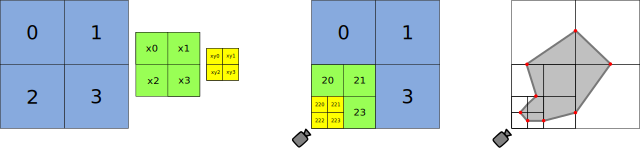
\includegraphics[width=0.9\textwidth]{figs/morton2}}
    %%\subfigure{}{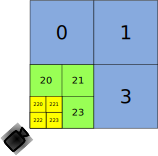
\includegraphics[height=0.17\textheight]{figs/partitioning}}
    %%\subfigure{}{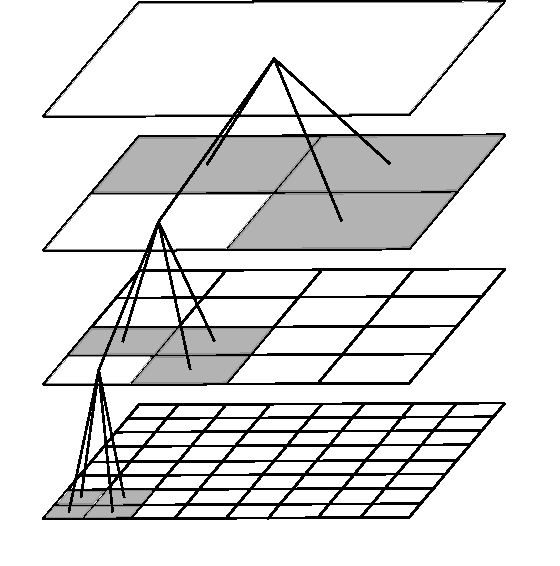
\includegraphics[height=0.17\textheight]{figs/quadtree_activefront}}
  \end{center}
\caption{Morton codes associated to cells of a linear quatree. Each
   morton code of a child cell is obtained by adding a suffix to its
  parent code \emph{(left)}. The adaptive representation consists of
  quadtree cells whose depth is view point dependent
  \emph{(middle)}. Finally, adaptive Marching Cubes is used to
  generate the triangulation \emph{(right)}.}
\label{fig_quadtree_partitionning}
\end{figure}

Representing a hierachical structure on GPU is usually challenging since
the GPU is a data parallel component and is unable to handle recursivity.

%since the GPU
%memory is limited and non consistent %\todo{fix coherent/aligned/coalesced?}
%memory access (\emph{e.g.} tree traversal using pointer dereferencing) may lead
%to huge payload from cache misses.

Efficient spatial tree encoding can be
achieved using pointerless structures such as linear quadtrees or octrees ( see
for instance \textsc{Gargantini}~\cite{gargantini1982effective} ). This structure
%consists in indexing each cell by a \emph{Morton code}: the code of children
indexes each cell by a \emph{Morton code}: the code of children
cells are defined by the code of the parent suffixed by two bits (in dimension
2, three bits in dimension 3) (see Figure
\ref{fig_quadtree_partitionning}-\emph{left}). A cell's code encodes its
position \wrt its parent cell and its complete path to the tree root.
%Hence, whatever their depth, all cell codes are simply stored in a linear vector on memory.
Hence, the tree is fully represented as a linear vector of its leaves, whatever their depth.
Furthermore, cell operations such as subdivision, merging, neighbors
access can be efficiently implemented using bitwise operations on the Morton
code. In the following, we use the GPU implementation proposed by \textsc{Dupuy}
\textit{et al.}~\cite{dupuy2014quadtrees} that we extended to the third dimension.
By using their approach, Morton codes
and bitwise operations are optimized to match with GPU hardware requirements.

\subsection{Data parallel and adaptive mesh generation}

Using this spatial data structure, triangulated mesh can be constructed
from a Marching Cubes approach \cite{lorensen1987marching} (MC for short): the
triangulation is generated from local triangle patches computed on
local cell configurations. Since triangle patches are locally
computed, such approach is fully parallel and easy to implement on GPU
hardwares. However, since adjacent cells may not have the same depth
in the octree, original \textsc{Lorensen} and \textsc{Cline}'s rules need to be
updated (see Figure~\ref{fig_quadtree_partitionning}-\emph{right}). Many authors have addressed this problem both for primal and
dual meshes
\cite{shu1995adaptive,schaefer2004dual,lengyel2010voxel,DBLP:journals/cgf/LewinerMPPL10,DBLP:journals/cvgip/LobelloDD14}.

In the following, we use the extension of MC configurations to handle
adaptive structures proposed by \textsc{Lengyel} \emph{et al.}~\cite{lengyel2010voxel}.
First, this approach constrains the octree
structure in order to make sure that the depth difference between any
two adjacent cells is at most one.
Then, \textsc{Lengyel} \emph{et al.} introduce the concept of transition cells.
Those cells are defined to be inserted between two neighbouring octree cells of different depth.
With specific MC configurations for such transition cells, a crack free triangulation can
be extracted.
%Then, \textsc{Lengyel} \emph{et al.} propose
%specific MC configurations for such transition cells,  leading to a
%crack-free triangulation.

Similarly to original MC algorithm, this approach is perfectly adapted
to GPU hardwares: Given a set of cells (a vector of morton codes),
each triangle patch can be constructed in parallel (done by
the \emph{geometry shader} in the GPU graphic pipeline).

\subsection{Level of Details Criteria and Temporal Updates}


As illustrated in Figure~\ref{fig_quadtree_partitionning}-\emph{middle}, we
propose a viewpoint dependent criterion to decide if a cell needs to be refined:
the closer we are to the camera, the finer the cells are.
%In addition to the
%distance criterion, we define an angular criterion to prevent refining cells
%outside the camera frustrum.
Using a criterion based on the distance between a
cell and the camera is well suited to GPU since it can be evaluated
independently on all cells. Hence, we can efficiently determine if a cell must
be subdivided or not. Figure~\ref{fig_lod_octree} illustrates the level of
details (LoD for short) criterion we use. More precisely, in dimension 2, if
$\alpha$ denotes the viewing angle, an object at distance $d$ from the camera
with diameter greater than $2\cdot d\cdot\tan(\alpha)$ is projected into more
than one pixel (see Figure~\ref{fig_lod_octree}-\emph{left}). Hence, the
distance criterion is based on the ratio (\emph{visibility ratio} in the
following) between the cell diameter $l(c)$ (power of 2 depending on the depth),
and $2\cdot d_c\cdot\tan(\alpha)$, $d_c$ being the distance between the cell
center and the camera. For a given cell $c$, split and merge decision are based
on this visibility ratio:
%
\begin{itemize}
  \item $c$ is split if its children
cells have a visibility ratio greater than  constant $k$\,;
  \item $c$ and its sibling cells are merged if their parent cell $c'$ has a visibility ratio lower than $k$\;
  \item otherwise, the cell $c$ stays for the next frame.
\end{itemize}
%
\begin{figure}[!h]
  \begin{center}
    \begin{overpic}[width=3.5cm]{figs/criterion}
      \put(33,40){$\alpha$}
      \put(50,45){$d_c$}
      \put(95,65){$l(c)$}
    \end{overpic}~~~~~
    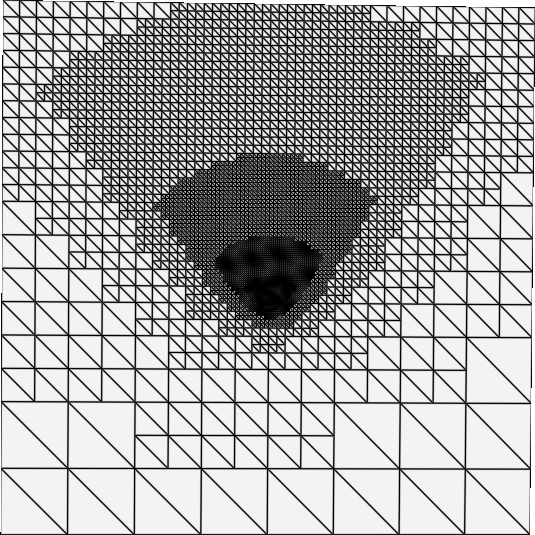
\includegraphics[width=3.5cm]{viewlod2_small}~~~~~
    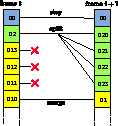
\includegraphics[width=3cm]{subdivision}
  \end{center}
  \caption{Notations \emph{(left)} and adaptive meshing in dimension 2 using the LoD distance and angular criterion \emph{(middle)}. Based on LoD criterion
    evaluation, the cell buffer is updated between each frame \emph{(right)}.}
  \label{fig_lod_octree}
\end{figure}
%
In addition to the distance criterion, we add an angular term in order
to prevent subdivision of cells far from the camera frustrum (see
Figure~\ref{fig_lod_octree}-\emph{middle}). We do not go into the
details but please note that stay, split and merge decisions of all cells are computed in
parallel from all cell morton codes.

Once decisions have been made, a new set of cells are sent to the mesh
generation step described above. Updating the cell buffer can be
efficiently implemented on GPU hardware as illustrated in
Figure~\ref{fig_lod_octree}-\emph{right}.  Finally, before
constructing the triangulation from remaining cells and transition
cells, geometrical culling is performed in order to skip the triangle
patch construction which are not visible. Figure~\ref{fig_pipeline}
illustrates the overall fully data parallel pipeline.

\begin{figure}[!htbp]
  \centering
  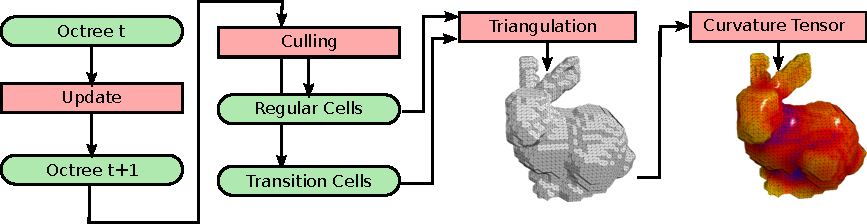
\includegraphics[width=0.9\textwidth]{figs/pipeline2}
  \caption{ Summary our GPU pipeline. Data buffers are
    represented in green and computations in red. Each computation
    retrieves data from a buffer and fills a new one. }
  \label{fig_pipeline}
\end{figure}




\section{Interactive Curvature Computation on GPU}
\label{sec:inter-visu-gpu}

We first present design principles for the GPU implementation and then
present our approaches.

\subsection{Design principles}

The general idea is to perform an Integral Invariant computation on
GPU at each vertex of the generated triangular mesh. First note that
when the LoD criterion is removed, each MC vertex is exactly centered at
a surfel center. At different depth of the octree, MC vertices still
correspond to surfel centers of subsampled versions of the input
object. Hence, Integral Invariant framework defined in
Section~\ref{sec:curv-tens-estim} is consistent with the triangular
surface obtained on GPU: triangles are used for visualization purposes
but all computations are performed on the digital object $\DSh$ and thus
estimators
(\ref{eq:dig-curvature-estimator-k}),
(\ref{eq:dig-curvature-estimator-H}), (\ref{eq:dig-curvature-estimator-k1})
and (\ref{eq:dig-curvature-estimator-k2}).

To implement the integration on $\Ball{R}{\vx} \cap \Shape$
(Fig.~\ref{fig:approx}-$a$), a naive approach consists in scanning all digital
points inside such domain (Fig.~\ref{fig:approx}-$b$) and then to estimate the
geometrical moment as the sum of the geometrical moments of each elementary
cubes lying in the intersection. On GPU, \emph{mipmap} textures are used to
obtain a multi-resolution information: if the input binary object is stored in a
3D texture, GPU hardware can construct a multi-resolution pyramid such that 8
neighboring voxel intensities at level $l$ are averaged to define the voxel
value at level $l+1$. If the level 0 corresponds to the binary input object, at
a given level $l$, a voxel $(x,y,z)$ contains the fraction of $\DSh$ belonging
to the cube of center $(x,y,z)$ and edge length $2^l$. As a consequence, we can
approximate the volume of $\Ball{R}{\vx}\cap\Shape$ by considering mipmap values
at a given resolution $l$ (Fig.~\ref{fig:approx}-$c$). In this case, errors only
occurs for cells lying inside $\Shape$ (with density 1) not entirely covered by
$\Ball{R}{\vx}$. Furthermore, the \emph{mipmap} texture can be used to design,
using a single texture probe, a fast inclusion test of a given cell $c$ at level
$l$ into the shapes: we say that $c$ is in $\Shape$ if its density (retrieved
from the texture probe at level l) is greater than $1/2$. The idea here is to
mimic a lend of adaptive Gauss digitization process.

\begin{figure}
  \begin{center}
    {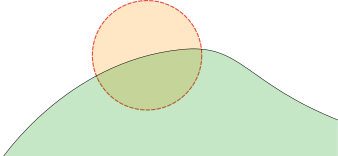
\includegraphics[width=4cm]{figs/approx1}}
    {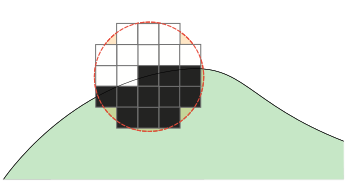
\includegraphics[width=4cm]{figs/approx-reg-1}}
    {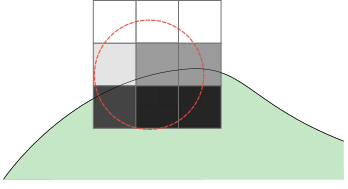
\includegraphics[width=4cm]{figs/approx-reg-2}}
  \end{center}
  \caption{Integral computation with an area estimation (\emph{left}) from pixel
    counting (\emph{middle}) or from densities (represented by different
    gray values) in a mipmap approximation of $\Shape$ (\emph{right}).}
  \label{fig:approx}
\end{figure}

Using the hierachical nature of the mipmap texture, we could also
consider hierarchical decompositions of either $\Ball{R}{\vx}$
(Fig.~\ref{fig:approx2}-$a$) or $\Ball{R}{\vx}\cap\Shape$
(Fig.~\ref{fig:approx2}-$b$). The idea would be to decompose the
regions into mipmap cells of different resolution in order to limit
the number of texture access (important bottleneck on GPU hardwares)
and to get better approximated quantities. Note that the scenario in
Fig.~\ref{fig:approx2}-$b$, is clearly the best approach: the
volume is exact  (\wrt the regular grid case) since geometrical moments
are additive quantities, and the number of texture fetches is  optimal
at this point.


\begin{figure}
  \begin{center}
    {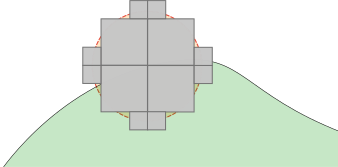
\includegraphics[width=4cm]{figs/approx-bh}}
    {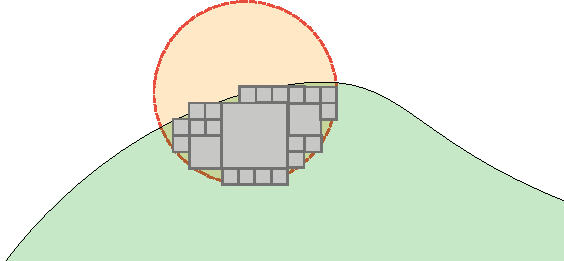
\includegraphics[width=4cm]{figs/approx-ada}}
  \end{center}
  \caption{Adaptive approximation of the integration using a
    hierarchical decomposition of the ball $\Ball{R}{\vx}$ (\emph{left}), or a decomposition of $\Ball{R}{\vx}\cap\Shape$ (\emph{right}).}
  \label{fig:approx2}
\end{figure}


\subsection{Per Vertex Real-time Computation on GPU}
\label{sec:hierarchical}

We describe here two different visualization pipeline on GPU that will
be evaluated in the next section.

\paragraph{Hierarchical Decomposition.}  As discussed above, best
results in terms of texture fetch can be obtained by the approach
presented in Fig.~\ref{fig:approx2}-$b$. At each vertex, the
computation algorithm would consist in a recursive decomposition of
the domain such that a cell is subdivided if it does not belong to
$\Ball{R}{\vx}\cap\Shape$. However, on GPU hardware, this approach is
highly inefficient since the hardware optimizes the parallelism only
when the micro-program described in the shader has a predictive
execution flow. Hence, implementing the recursive algorithm (or its
de-recursified version) requires a lot of branches (conditional
\emph{if} tests) in the flow. Instead of implementing this approach,
we have considered a fast hierarchical approximation following
Fig.~\ref{fig:approx2}-$a$: for a given radius $R$, we precompute a
hierachical decomposition of $B_R$. Such decomposition is made of
octree cells at different resolutions. At a given MC vertex $\vx$, the
algorithm becomes simple since we just scan the ball cells and
estimate the area (or other moments) from the mipmap values associated
to this cell. Note that cells in the $B_R$ decomposition may not be
aligned with mipmap cells. However, we can use GPU mipmap
functionalities which interpolates mipmap values if we probe at
non-discrete positions. For a given radius $R$, the expected number of
cells on $B_R$ is in $O(\log{R})$. Implementation details on the
hierarchical octree representation can be found in the supplementary
material (see Section \ref{sec:discussion}).


%\todo[inline]{phrase sur approx si on met}





\paragraph{Dynamic Refinement.} In this approach, we want to optimize
the interactivity and the execution flow or parallelism on GPU. The
integration is simply computed using a regular grid at different
resolution $l$ (Fig. \ref{fig:approx}-$b$ and $c$). The shader code
becomes trivial (simple triple loop) and a lot of texture fetched are
involved, but interactivity can be easily obtained. Indeed, we
consider the following multi-pass approach:
\begin{enumerate}
\item When the surface geometry has been computed,we set the current
  level $l$ at an high level $l\EqDef l_{max}$ of the mipmap
  pyramid.
\item We compute the integrals (and the curvature tensor) at the
  mipmap level $l$ and  send the estimated quantities to the
  visualization stage.
\item If the user changes the camera position or the computation
  parameters, we return to step 1.
\item If the current framerate is above a given threshold, we decrease
  $l$ and return to step 2 if the final $l_0$ level has not been
  reached yet.
\end{enumerate}
A consequence of the multi-pass approach is that is there is no
interaction (camera settings, parameters), the GPU automatically
refine the estimation. Even if step 2 is quite expensive, in
$O\left(\left(\frac{R}{2^l}\right)^3\right)$, the interactive control
 in step 3 considerably improves the interactive exploration of the
 tensor with fast preliminary approximations which are quickly refined.

 Compared to the hierarchical approach, no precomputation is required
 for a given radius $R$. As a consequence, we could even locally adapt
 the ball radius to the geometry (for instance following the octree
 depth of the current MC vertex). In the next section, we evaluate the
 performances of both approaches.


\section{Experiments}
\label{sec:experiments}

\subsection{Full resolution experiment}


\begin{figure}
  \begin{center}
    {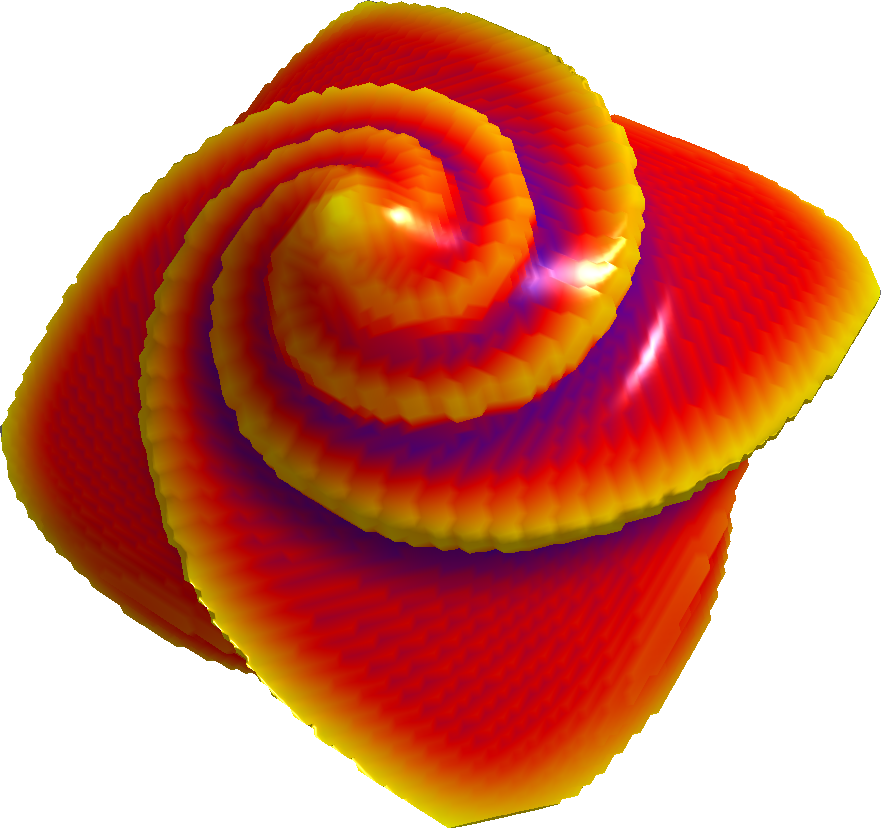
\includegraphics[width=2.2cm]{figs/Octa_mean}}
    {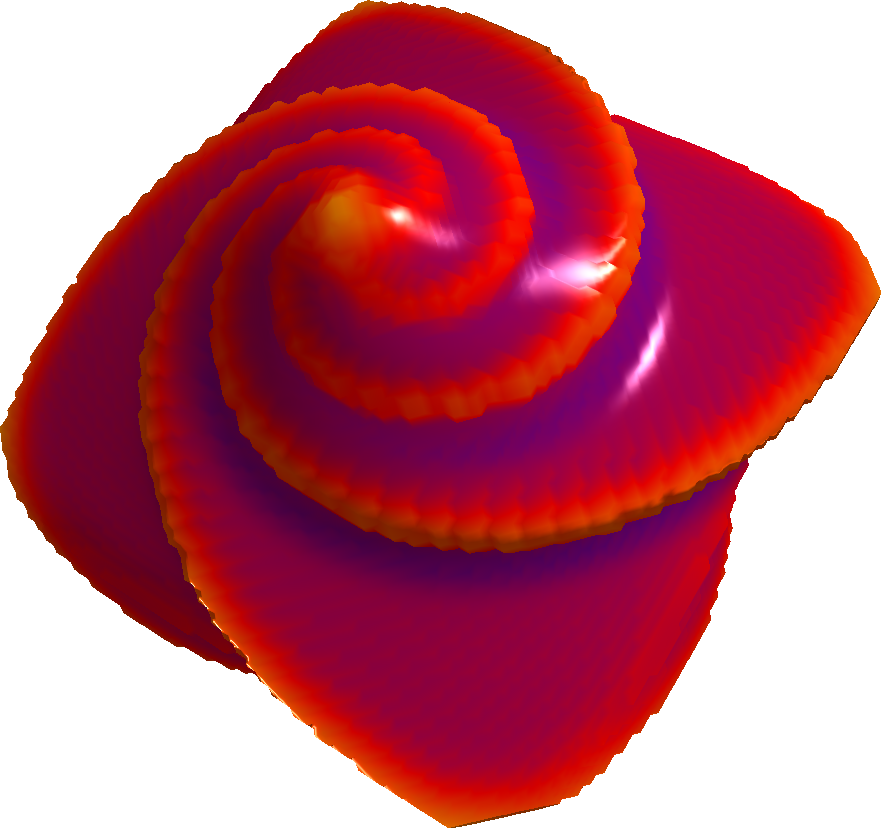
\includegraphics[width=2.2cm]{figs/Octa_gaussian}}
    % {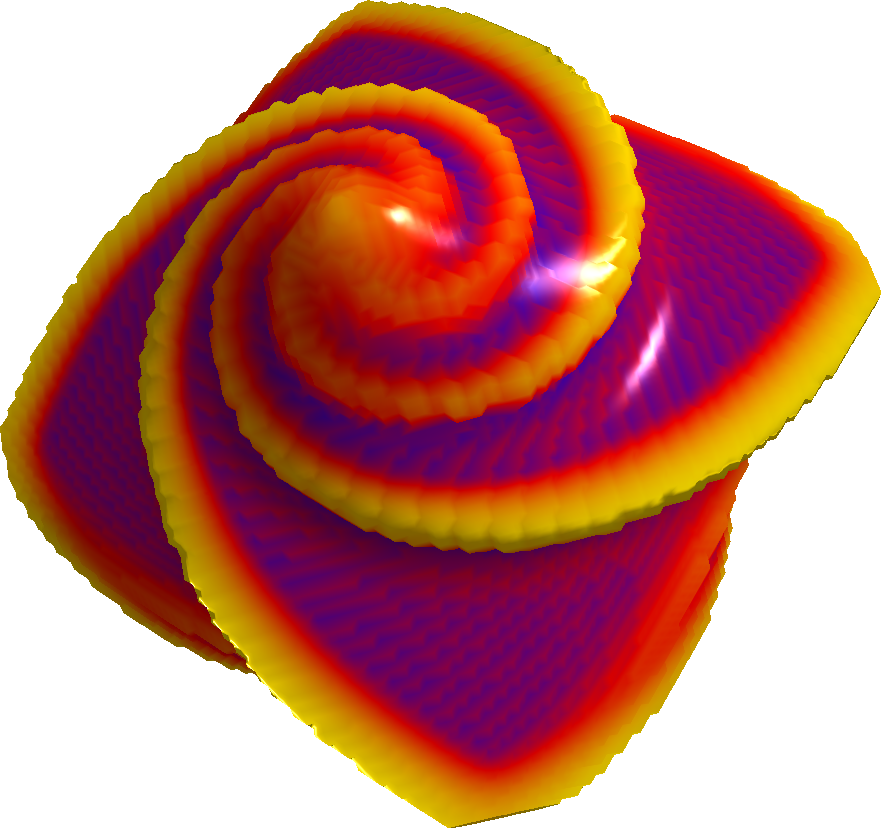
\includegraphics[width=2.7cm]{figs/Octa_k1}}
    % {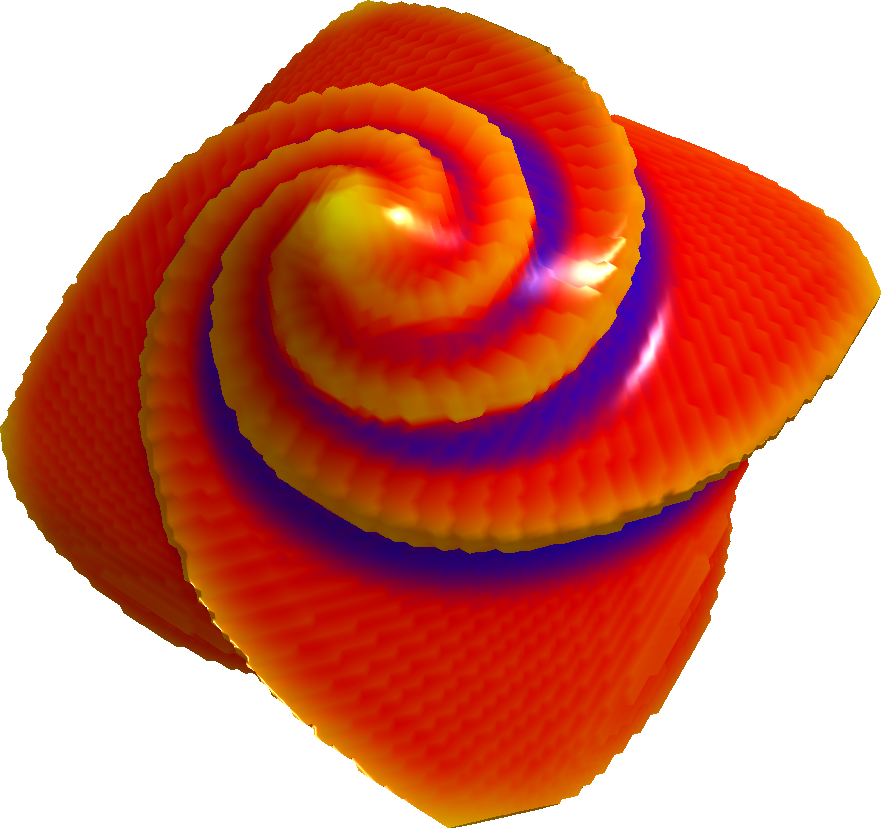
\includegraphics[width=2.7cm]{figs/Octa_k2}}\\
    % {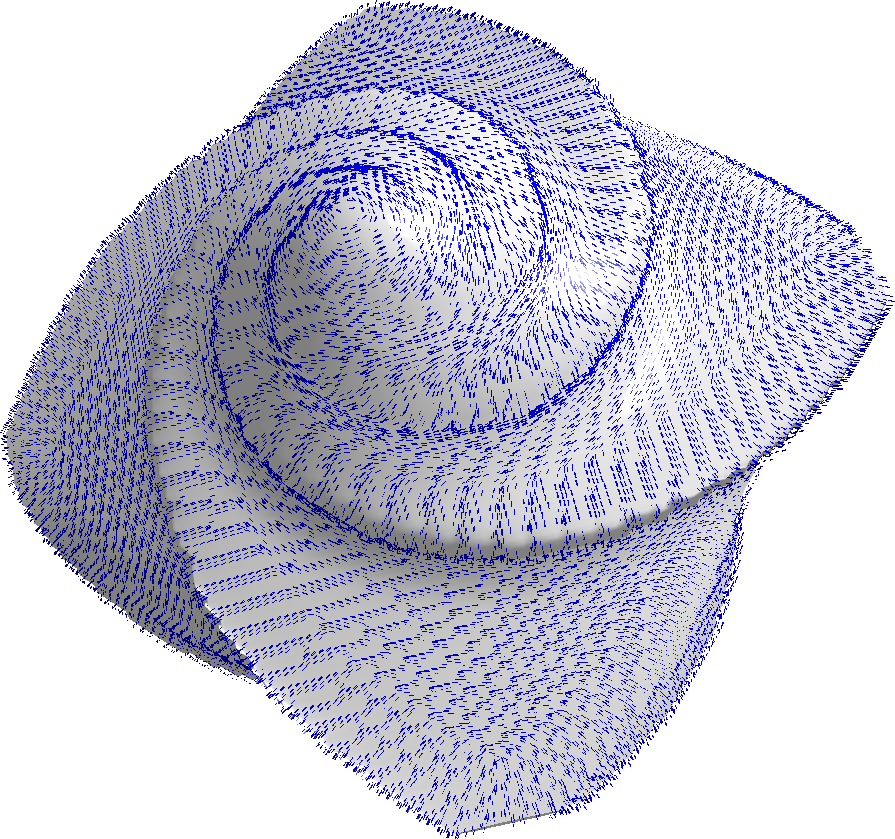
\includegraphics[width=2.7cm]{figs/Octa_dir_min}}
    % {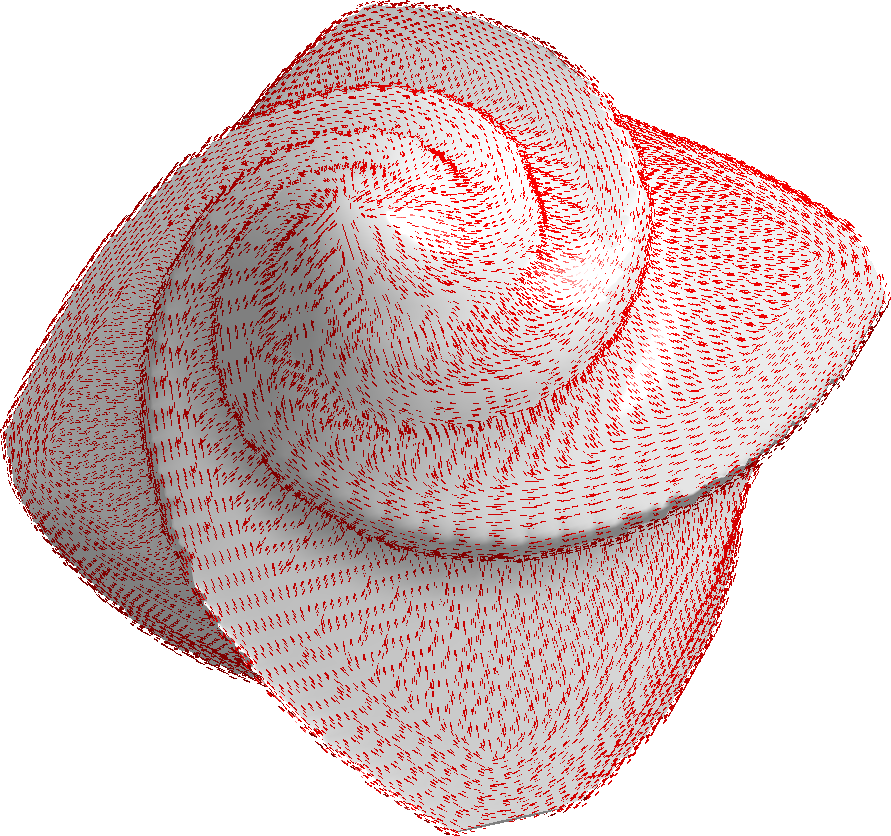
\includegraphics[width=2.7cm]{figs/Octa_dir_max}}
    {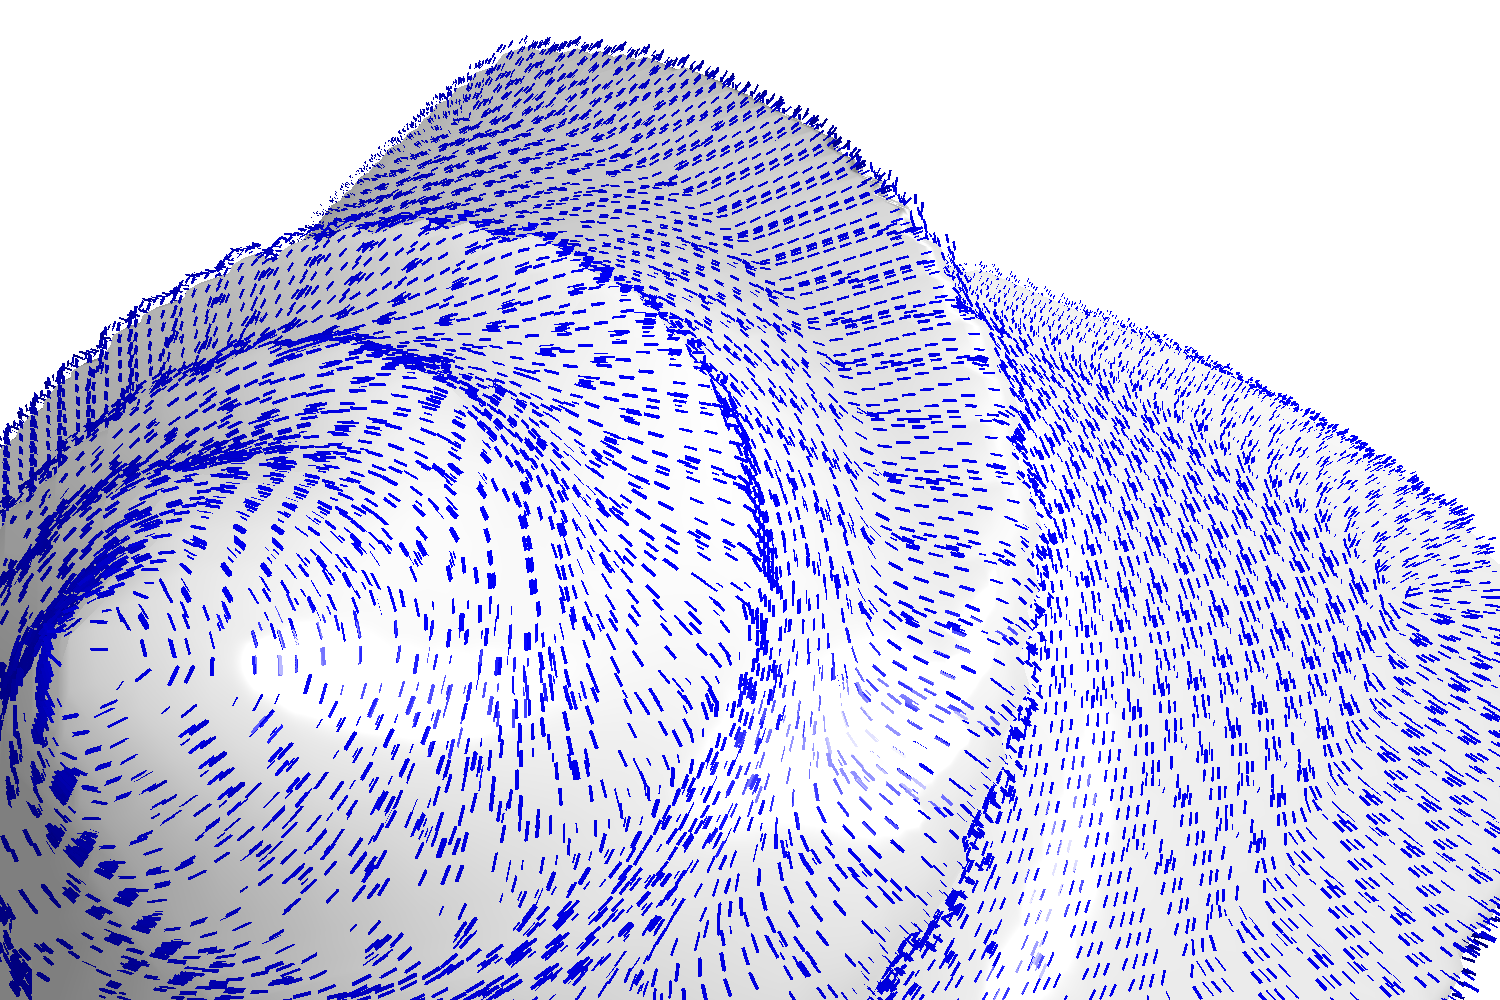
\includegraphics[height=2.0cm]{figs/Octa_dir_min_zoom}}
    {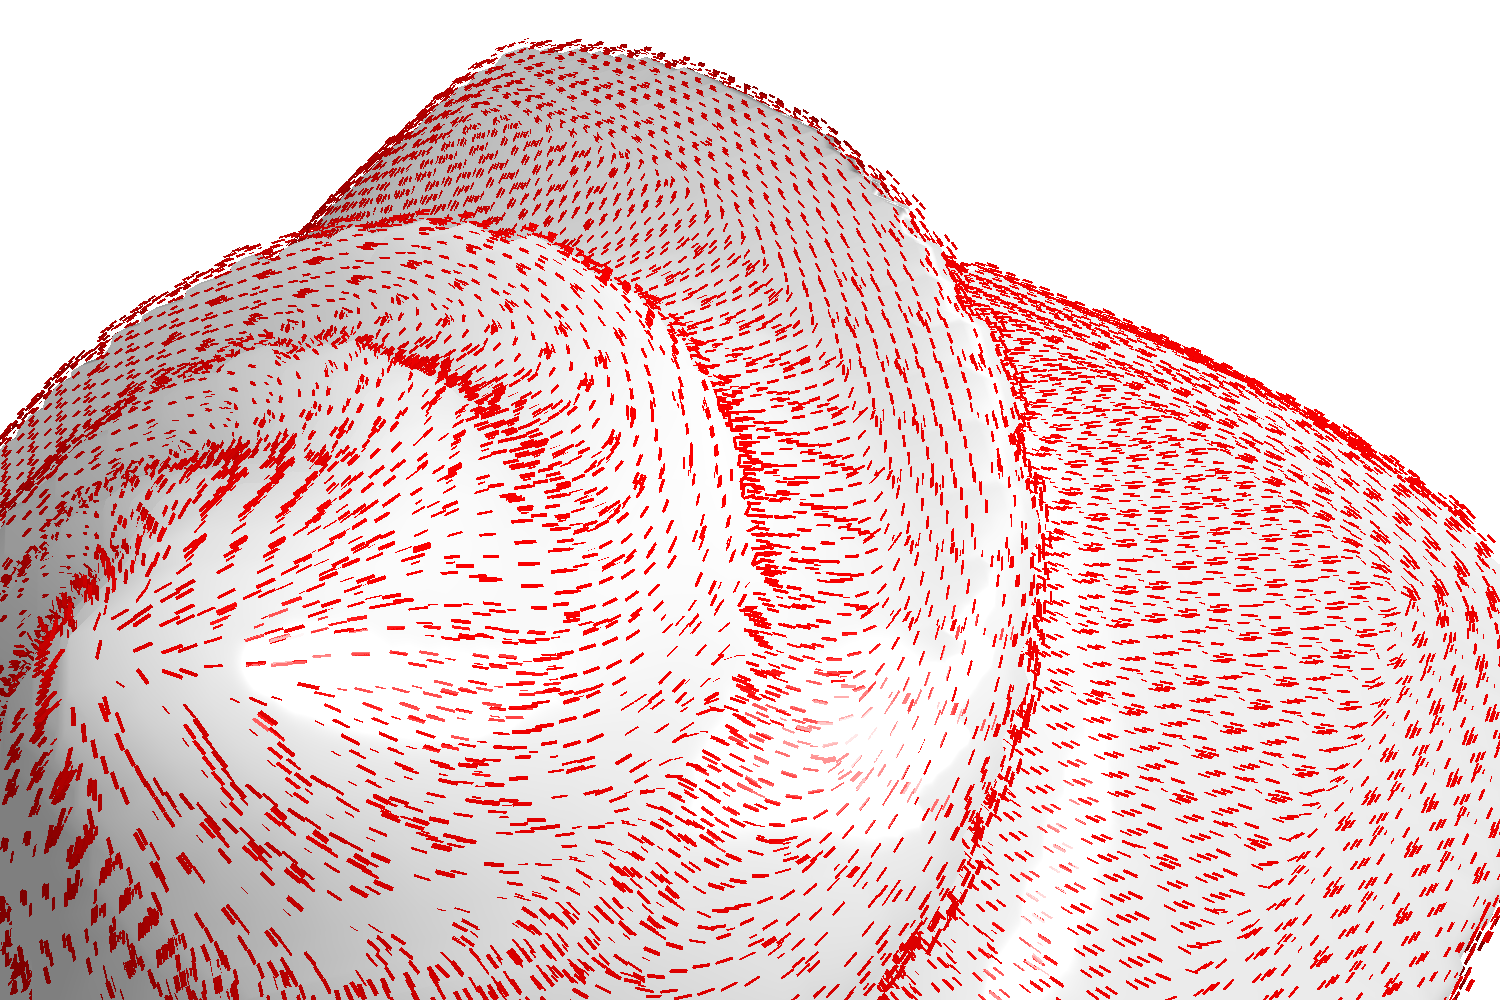
\includegraphics[height=2.0cm]{figs/Octa_dir_max_zoom}}\\
    % {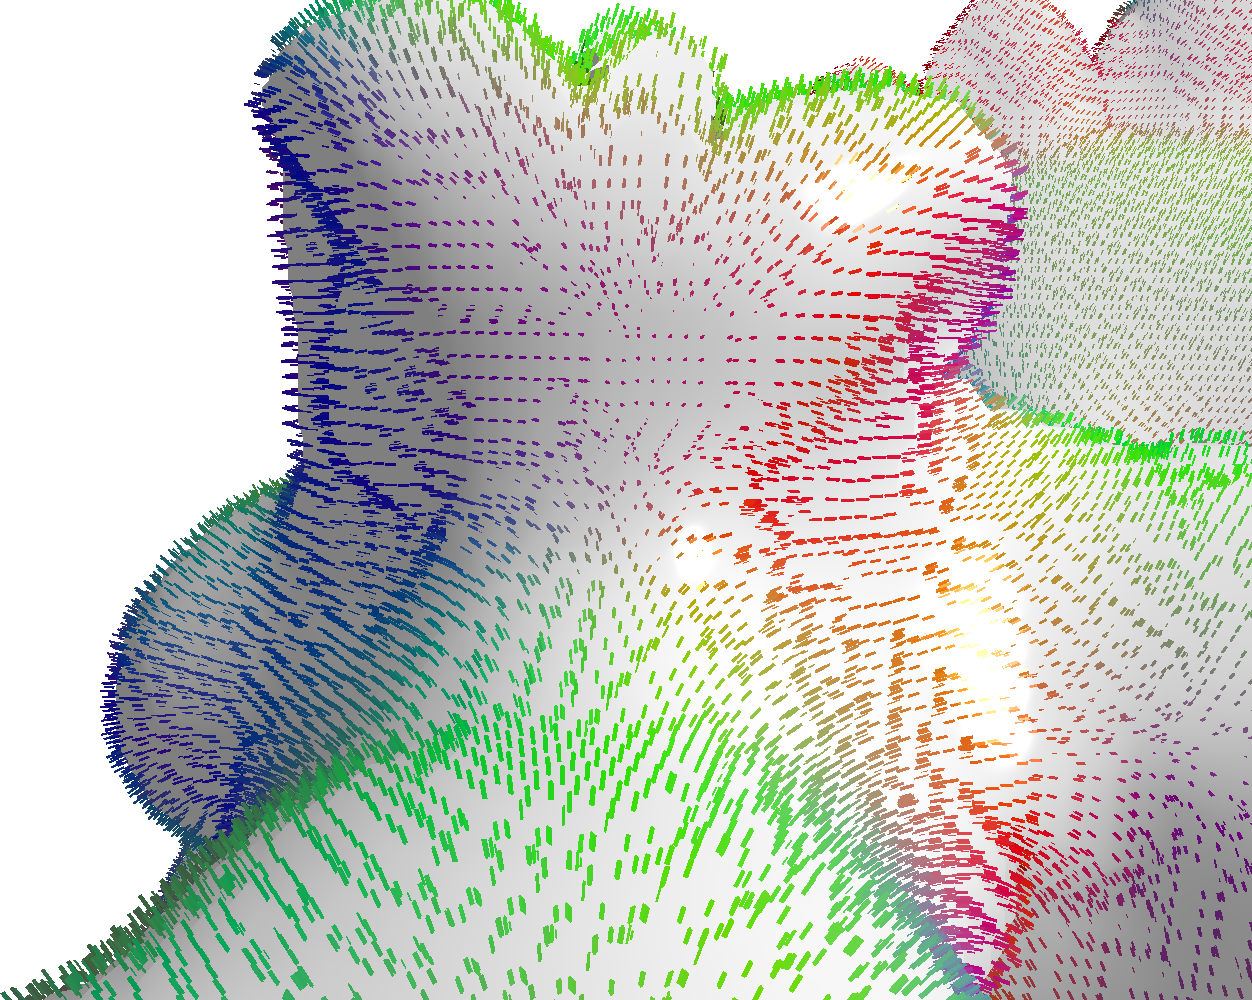
\includegraphics[height=4.0cm]{figs/EG_dragon_normal_zoom}}
    {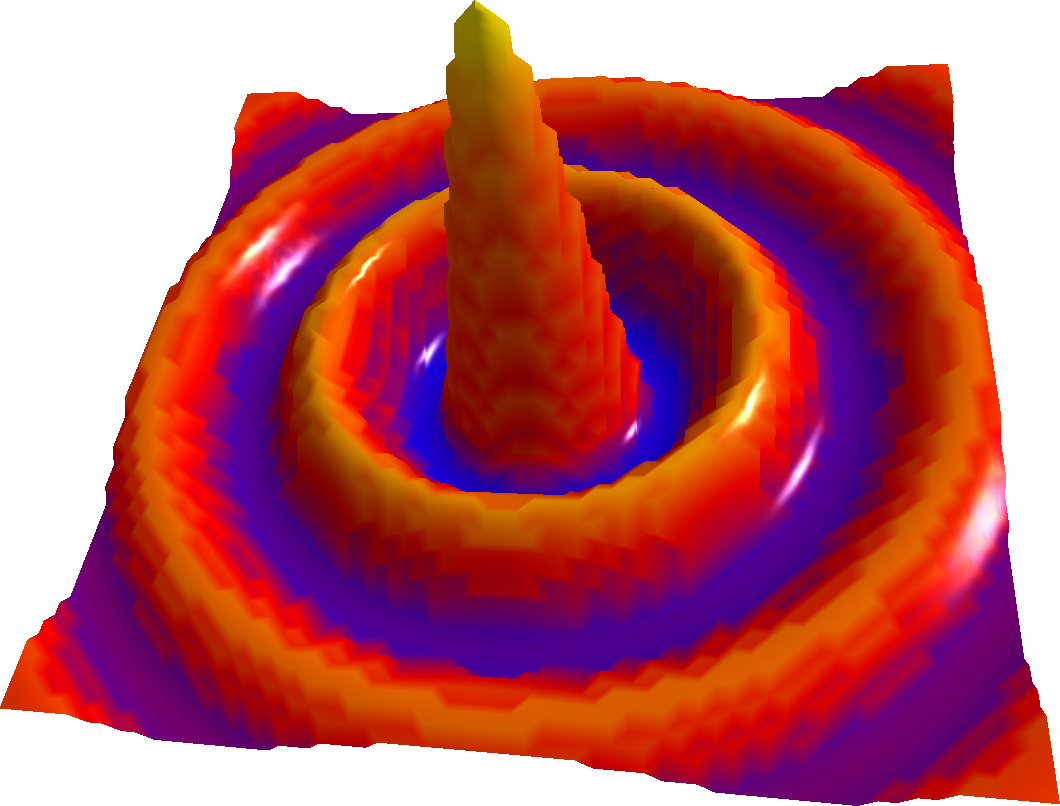
\includegraphics[width=2.2cm]{figs/function_mean_0}}
    {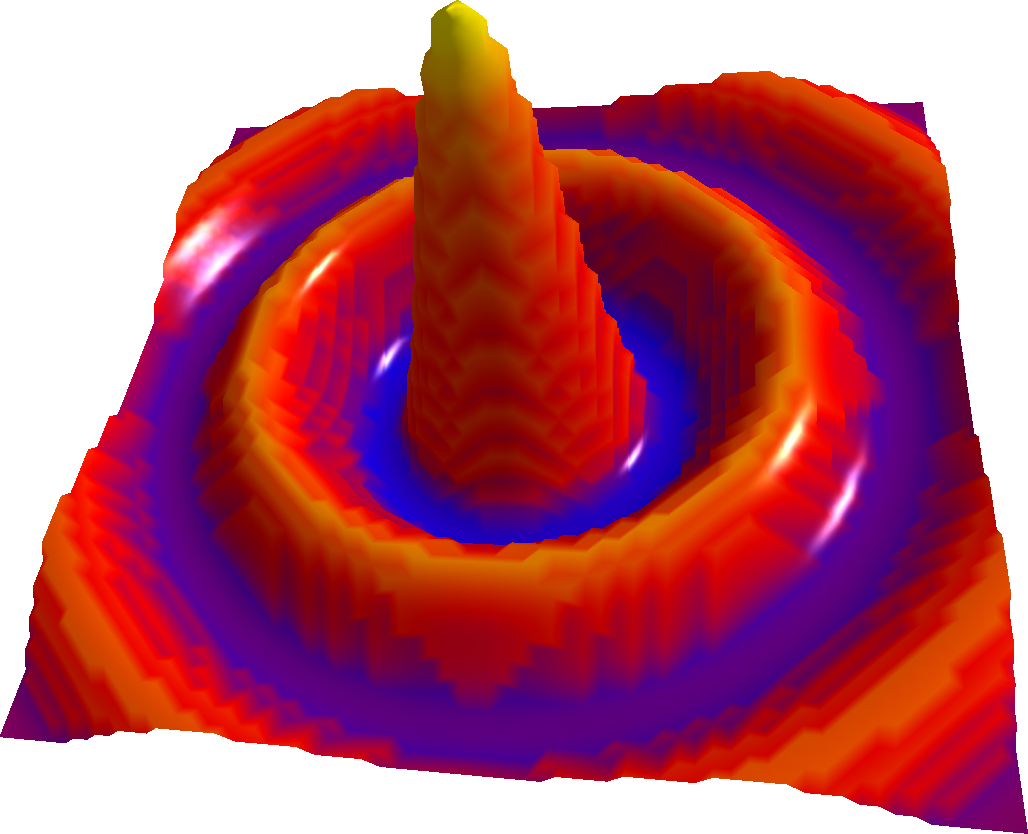
\includegraphics[width=2.2cm]{figs/function_mean_1}}
    {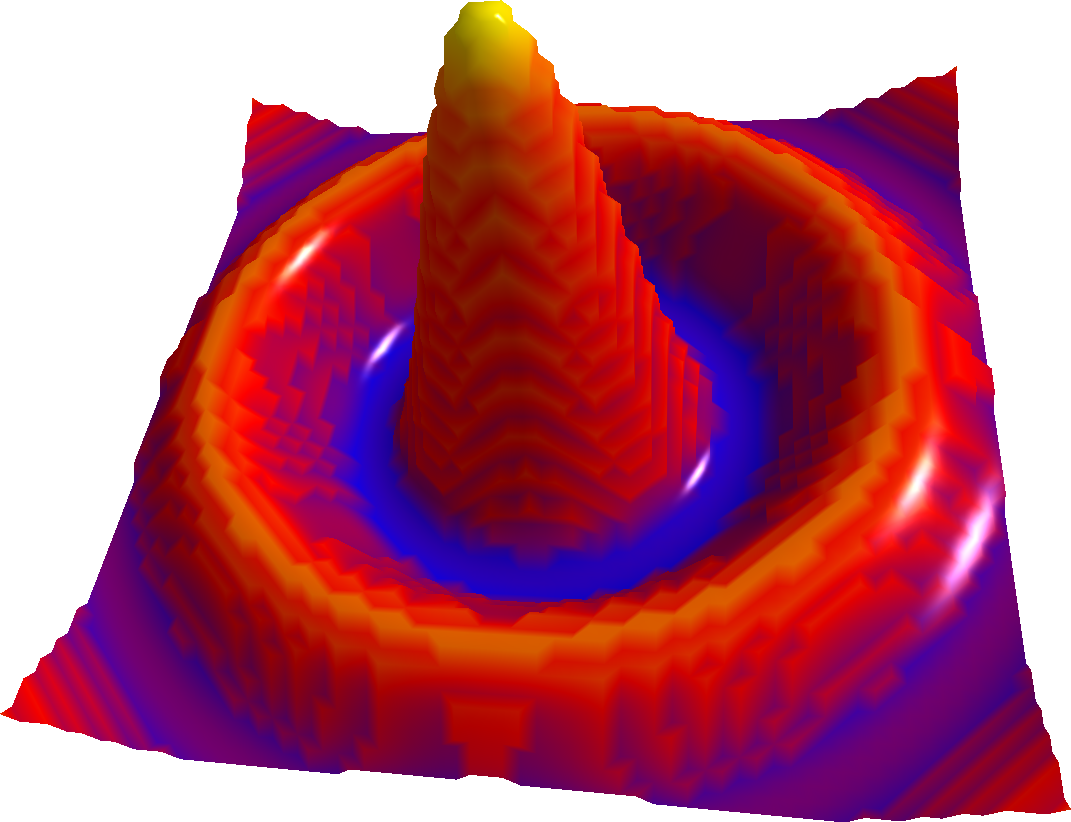
\includegraphics[width=2.2cm]{figs/function_mean_2}}
    {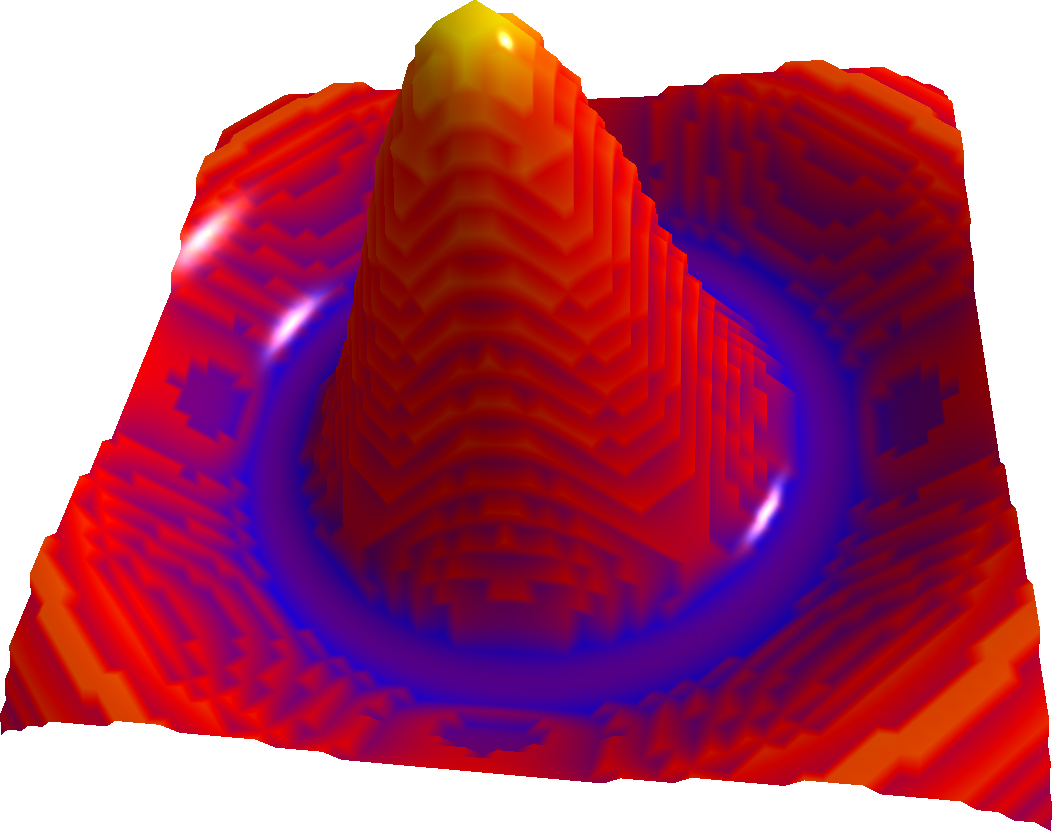
\includegraphics[width=2.2cm]{figs/function_mean_3}}
    {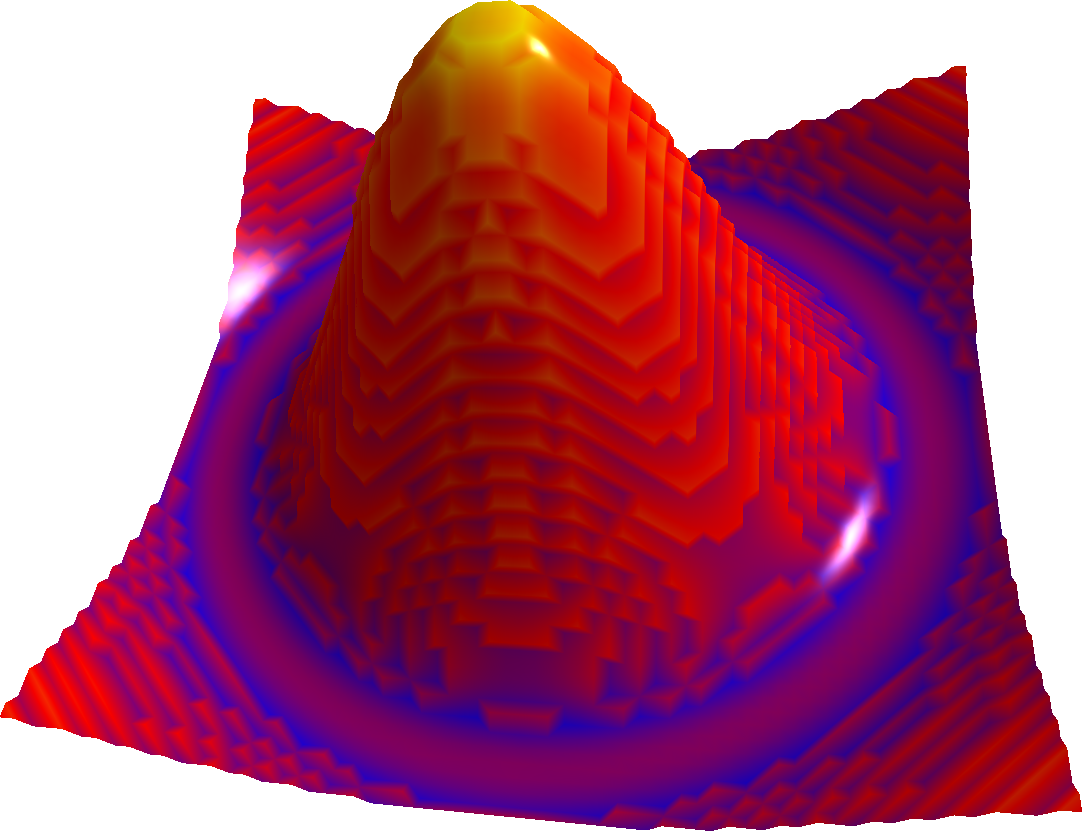
\includegraphics[width=2.2cm]{figs/function_mean_4}}
  \end{center}
  \caption{\emph{First row}: Mean and Gaussian curvature estimation, (zoom of) first and second principal directions estimation on an OctaFlower with a digital domain of $130^3$.
  % \emph{Second row:} (Zoom of) First and second principal directions estimation on an OctaFlower.
  \emph{Third row:} Mean curvature computed in real-time on a dynamic object.}
  \label{fig:full}
\end{figure}

\begin{figure}
  \begin{center}
    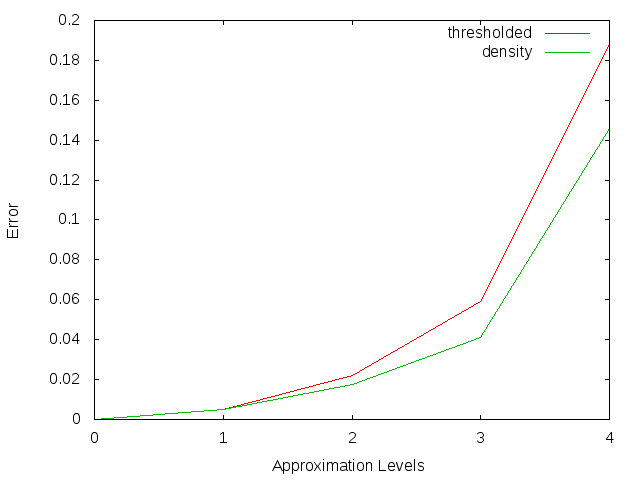
\includegraphics[width=0.5\textwidth]{figs/graph_cmp_l0_l4_mean_octa130_Linf}
  \end{center}
  \caption{Error $L\infty$ on the measured Mean curvature between a $l_n$ approximation and the
  $l_0$ measurement. The red curve present the results when computing the volume from a mipmap quantitized to 0 or 1, and the green one
  present the results when computing it from the real mipmap values.}
  \label{fig:graph_convergence}
\end{figure}

We first evaluate the curvature estimation on a full-resolution geometry
obtained by disabling the LoD criterion at the mesh generation step.
Figure~\ref{fig:full}-top and middle shows results of curvature tensor
estimation (mean, Gaussian, first and second principal curvatures, first and
second principal directions) on an OctaFlower at level $l_0$ (ground truth).
Figure~\ref{fig:full}-bottom shows mean curvature estimation in real-time on a
dynamic object. For this case, we simply evaluate the implicit expression at
each vertex of a cell to decide if such cell is included or not into
$\Ball{R}{\vx}\cap \Shape$ instead of updating the \emph{mipmap texture} of
densities at each time step. For all illustrations, we use directly normal
vectors computed by algorithm discussed in Section~\ref{sec:curv-tens-estim}.

Then, we compare the approximation made by computing curvature from level $l \ge
l_0$ in Figure~\ref{fig:refine}. We can see that results using approximation
seems to fastly converge to the ground truth results.
Table~\ref{tab:full-res-stat} shows numerical results of $L_\infty$ error (worst
case) and $L_2$ error (mean), as well the number of \emph{mipmap texture}
fetches. We can first see that the number of texel fetch required to compute the
curvature reduces drastically when computing the approximations. This is
mandatory if we want to increase the framerate.


 in order to accelerate visualisation with the ground truth result obtained
at level $l_0$. We also compare them with the hierarchical algorithm discussed
in Section~\ref{sec:hierarchical}. The results are presented in
Table~\ref{tab:full-res-stat}, and illustrated in Figure~\ref{fig:refine}.


However, we can also note that the error increases quite slowly.
The errors obtained comparing $l_1$, or for bigger radii $l_2$ approximations
with the $l_0$ level are small. The errors measured comparing higher levels
are of course much bigger and those level are thus never used in practice.
They are presented here to illustrate how the refining process converges to
the $l_0$ level.

This convergence is shown in Figure \ref{fig:convergence}. It has been evaluated using
two different strategy for volume computation. The first one reads the interpolated
data from the mipmap is adds 1 to the volume if this value is above a threshold.
The second strategy adds directly to the volume the interpolated data read from the mipmap.
The results are shown Figure \ref{fig:graph_convergence}. It can be seen that the
interpolation done by the mipmap allows the resulting curvature to converge
faster to the $l_0$ level.

Thanks to this low error, higher approximation levels are visually
very similar to the $l_0$ level. We can therefore use them for exploring our
datasets in real time, changing the radii on the fly and visualising dynamic datasets.

When computing results using the hierachical algorithm, a higher error can be noted.
This is due to the precomputation of the subdivision that no longer ensures to fetch data
at the center of a mipmap cell. The interpolation done by the GPU reduces the bias but
does not remove it.

Bear also in mind that those results were measured on a full resolution triangulation.
Since we compute the curvature of each vertices of the final mesh, a highly triangulated object will
be much slower to process.
We therefore use in practice an adaptive triangulation of the object, refining the mesh
when it is closer from the camera and thus reducing the number of vertices to compute.

\begin{table}
  \begin{center}
  \setlength{\tabcolsep}{0.15cm}
	\begin{tabular}{@{}llrrrrrr@{}}
      \toprule
        & & H & $l_4$ & $l_3$ & $l_2$ & $l_1$ & $l_0$\\
      \midrule
      \multirow{2}{2.2cm}{Number of texture fetches} & $R=8$ & 1468 & & 2 & 28 & 260 & 2104 \\
                                & $R=16$ & 5706 & 2 & 28 & 90 & 2120 & 17080\\\midrule

      \multirow{2}{2.2cm}{$L_\infty$ error (\wrt $l_0$)} & $R=8$ & 0.051 & & 0.306 & 0.085 & 0.047 & 0\\
                                    & $R=16$ & 0.053 & 0.146 & 0.041 & 0.017 & 0.005 & 0\\\midrule

      \multirow{2}{2.1cm}{$L_2$ error (\wrt $l_0$)} & $R=8$ & 3.51e-05 & & 2.67e-04 & 7.57e-05 & 2.02e-05 & 0\\
                               & $R=16$ & 4.43e-05 & 1.39e-04 & 4.16e-05 & 1.57e-05 & 2.07e-06 & 0\\
      \bottomrule
    \end{tabular}
  \end{center}
  %
  \caption{Comparison of number of texture fetches, $L_2$ and $L_\infty$ error
  obtained on OctaFlower with a digital domain of $130^3$ when computing mean
  curvature with two radii: 8 and 16, with hierarchical algorithm (H) and $l \ge
  l_0$ approximation algorithms. The object is triangulated at full resolution
  with a regular grid and contains 282,396 vertices.
  %
  \label{tab:full-res-stat}}
  %
\end{table}

\begin{figure}[!htbp]
  \begin{center}
   {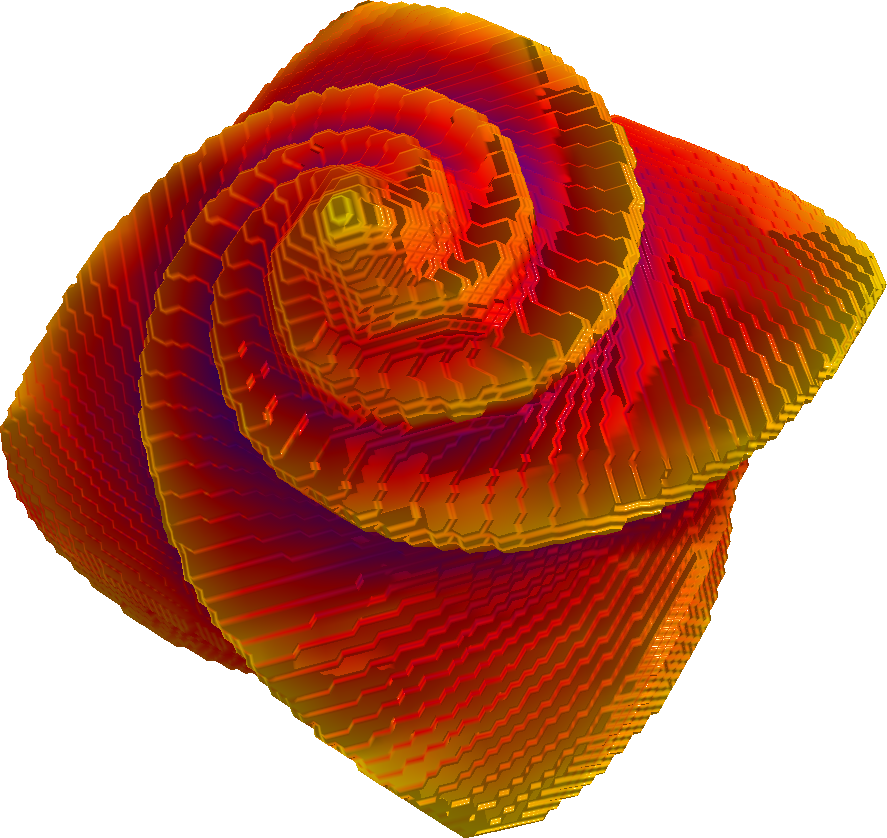
\includegraphics[width=2.7cm]{figs/octa_r10_l3_a}}
   {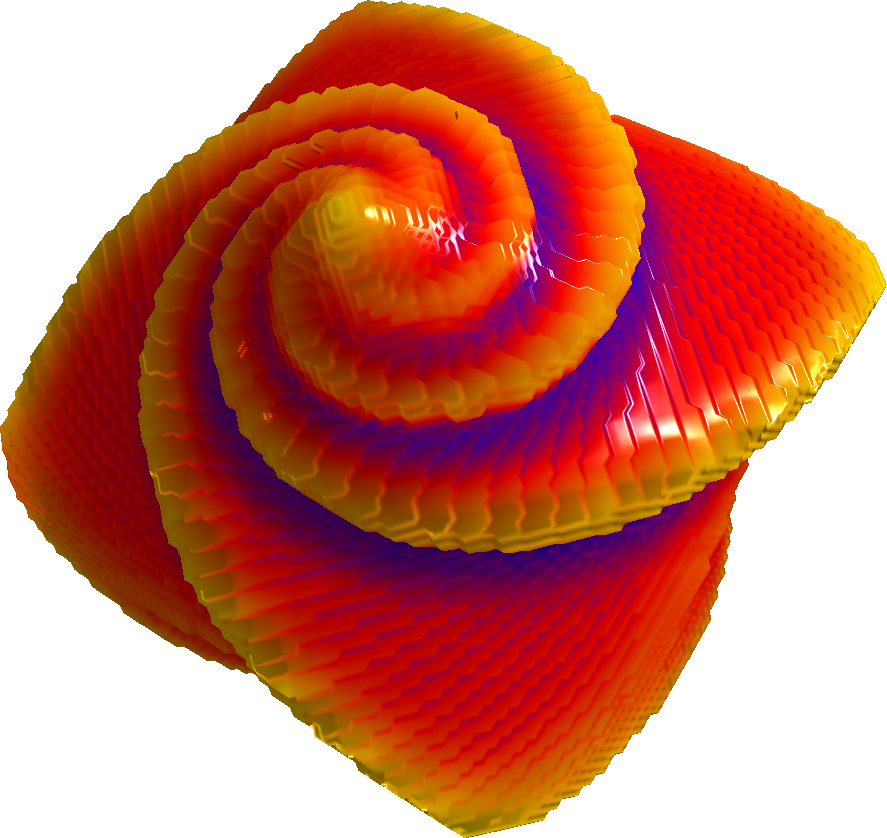
\includegraphics[width=2.7cm]{figs/octa_r10_l2_a}}
   {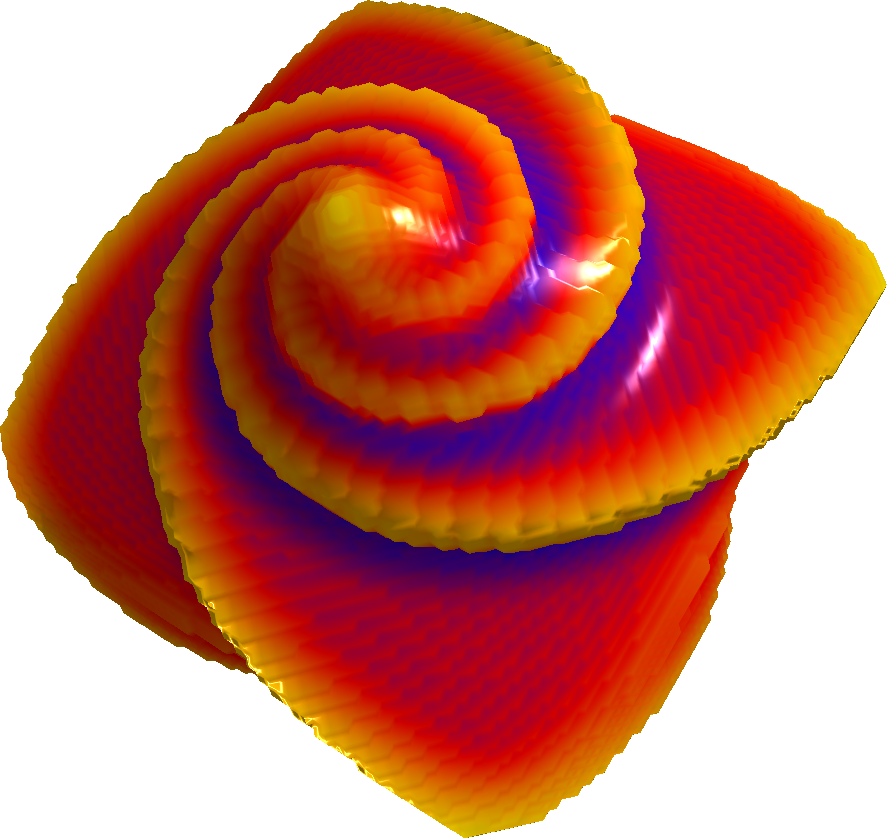
\includegraphics[width=2.7cm]{figs/octa_r10_l1_a}}
   {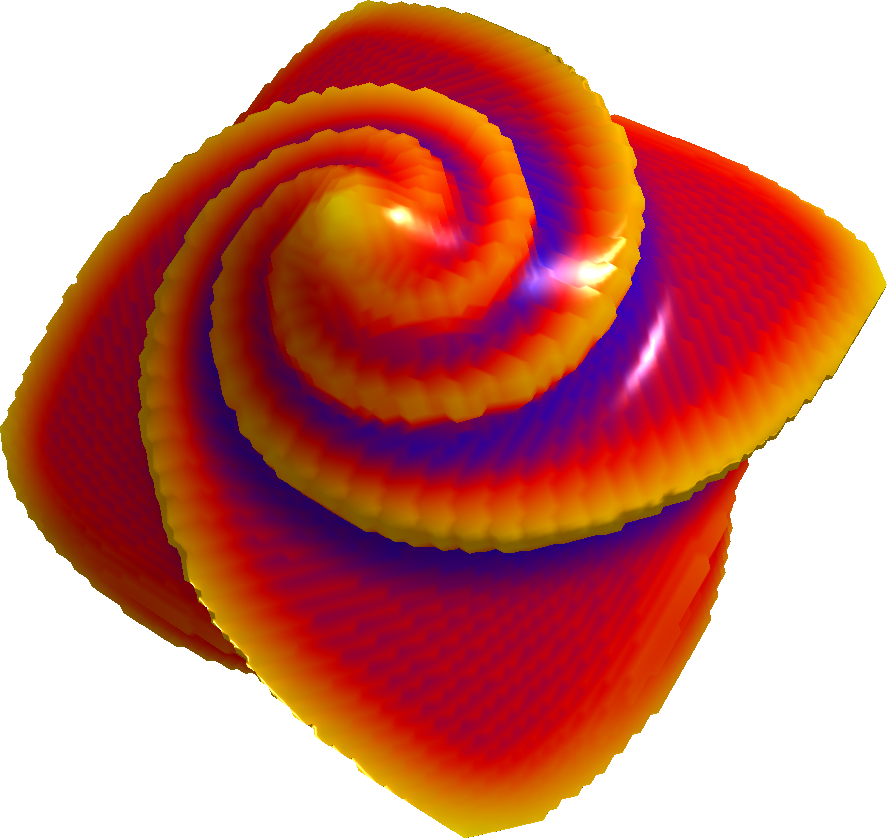
\includegraphics[width=2.7cm]{figs/octa_r10_l0_a}}
  \end{center}
  \caption{Illustration of mean curvature computation on an OctaFlower (digital domain of $130^3$) using mipmap approximation with different levels : $l_3$, $l_2$, $l_1$ and $l_0$ (\ie no approximation).
  %
  For all illustrations, we use directly normal vectors computed by algorithm discussed in Section~\ref{sec:curv-tens-estim}}
  \label{fig:refine}
\end{figure}


\subsection{Fully adaptive evaluation}

\begin{figure}[!htbp]
  \begin{center}
    \begin{tikzpicture}[scale=0.7]
      \begin{axis}[
          ybar stacked,
          ymode = log,
          ymax = 6000,
	  	  bar width=20pt,
	  	  nodes near coords,
	  	  every node near coord/.style={ font=\tiny, inner sep=0pt},
          enlargelimits=0.15,
          ylabel={\#Time (in ms)},
          symbolic x coords={Octa-R8, Octa-R16, Snow-R10, Snow-R20,
	      Dragon-R8, Dragon-R20},
          xtick=data,
          point meta=rawy,
          x tick label style={rotate=45,anchor=east},
        ]
        %Geometry Generation
        \addplot+[ybar, color=black, fill=cgeometry] plot coordinates {(Octa-R8,17.283000) (Octa-R16,18.458000)
          (Snow-R10,9.831000) (Snow-R20,9.653000)  (Dragon-R8,136.300000) (Dragon-R20,145.450000)};
        %l4
        \addplot+[ybar, color=black, fill=clquatre] plot coordinates {(Octa-R8,1) (Octa-R16,2.509000)
          (Snow-R10,6.085000) (Snow-R20,9.445000)  (Dragon-R8,3.389000) (Dragon-R20,20.228000)};
        %l3
        \addplot+[ybar, color=black, fill=cltrois] plot coordinates {(Octa-R8,2.527000) (Octa-R16,4.159000)
          (Snow-R10,10.629000) (Snow-R20,11.542000) (Dragon-R8,20.397000) (Dragon-R20,26.710000)};
        %l2
        \addplot+[ybar, color=black, fill=cldeux] plot coordinates {(Octa-R8,3.783000) (Octa-R16,9.006000)
          (Snow-R10,13.777000) (Snow-R20,37.700000) (Dragon-R8,29.967000) (Dragon-R20,92.435000)};
        %l1
        \addplot+[ybar, color=black, fill=clun] plot coordinates {(Octa-R8, 11.004000) (Octa-R16,38.687000)
          (Snow-R10,39.627000) (Snow-R20,217.954000) (Dragon-R8,59.840000) (Dragon-R20,506.549000)};
        %l0
        \addplot+[ybar, color=black, fill=clzero] plot coordinates {(Octa-R8, 37.273000) (Octa-R16,244.353000)
          (Snow-R10,236.194000) (Snow-R20,1655.680000) (Dragon-R8,322.674000) (Dragon-R20,3763.422000)};
        %\legend{\strut Geometry, \strut Curvature, \strut xx, \strut xx}
      \end{axis}
	  \end{tikzpicture}
%
    \begin{tikzpicture}[scale=0.7]
      \begin{axis}[
          ybar stacked,
          ymax = 6000,
          ymode = log,
	  	  bar width=20pt,
	  	  nodes near coords,
	  	  every node near coord/.style={ at={(0,0)}, font=\tiny, inner sep=0pt},
          enlargelimits=0.15,
          %ylabel={\#Time (in ms)},
          symbolic x coords={Octa-R8, Octa-R16, Snow-R10, Snow-R20,
	      Dragon-R8, Dragon-R20},
          xtick=data,
          point meta=rawy,
          x tick label style={rotate=45,anchor=east},
        ]
        %Geometry Generation
        \addplot+[ybar,color=black, fill=cgeometry] plot coordinates {(Octa-R8,17.283000) (Octa-R16,17.183000)
          (Snow-R10,9.383000) (Snow-R20,9.767000)  (Dragon-R8,127.347000) (Dragon-R20,127.166000)};
        %Hierarchical measurement
        \addplot+[ybar, color=black, fill=clzero] plot coordinates {(Octa-R8,18.095000) (Octa-R16,64.186000)
          (Snow-R10,96.747000) (Snow-R20,364.547000)  (Dragon-R8,147.662000) (Dragon-R20,787.459000)};
        %\legend{\strut Geometry, \strut Curvature, \strut xx, \strut xx}
      \end{axis}
     \end{tikzpicture}
     \end{center}
  %
  \caption{Timings in milliseconds (in logscale) obtained while visualizing an adaptive
  triangulation on three objects -- OctaFlower (digital domain of $130^3$ ), Snow
  Microstructures ($233^3$) and XYZ-Dragon ($510^3$) --  by computing the
  curvature with a regular grid (\emph{left}) and with hierarchical
  algorithm (\emph{right}), with two different radii for each object.
  %
  In \emph{orange color}: time required to extract the triangulation.
  %
  In \emph{blue color}: time required to compute the curvature tensor at
  different levels: from $l_4$ (light blue) to $l_0$ (dark blue).
  %
  Timings are given using a NVIDIA GeForce GTX 850M GPU.
  }
  %
  \label{fig:timings}
\end{figure}

When dealing with large datasets, we can not expect real-time curvature tensor
estimation due to the huge amount of data to process. By computing an
dynamically refined approximate curvature tensor estimation joined with an
adaptive triangulation (as discussed in Section~\ref{sec:hierarchical}), we
manage to maintain a real time framerate by giving control over the amount of
data to process at each frame. In Figure~\ref{fig:timings}, we compare timings
(in logarithmic scale) when the triangulation is dynamically refining according
to its distance to the camera. We measured those timings using the regular and
the hierarchical algorithm.

We can first note that the required time for an object to compute ground truth
curvature is usually as high as the time required to extract the geometry and
compute all the above levels. Using approximations is thus mandatory, since for
big objects such as the XYZ-Dragon ($510^3$) with big radii the approximate
computation is faster than the $l_0$ while results are close enough. For
example, with $R=20$, the approximated visualization at $l_2$ takes only 300ms
while the $l_0$ visualization takes more than 4 seconds.

We can thus get an approximated visualisation of our object as soon as we run
the application, allowing for real time interactions with the object (changing
the visualized value, curvature radius, \ldots). It is also clear on those
graphs that using a hierarchical decomposition reduces the curvature computation
time, especially with big radii. For the XYZ-Dragon with $R=20$, it needs almost
4 seconds to compute the $l_0$ level, whereas using the hierarchical algorithm,
it only needs 700ms. However, due to the precomputation and current hierarchical
structure, this algorithm is biased and creates an error (presented in
Table~\ref{tab:full-res-stat}) that needs to be considered.

\begin{figure}
  \begin{center}
    {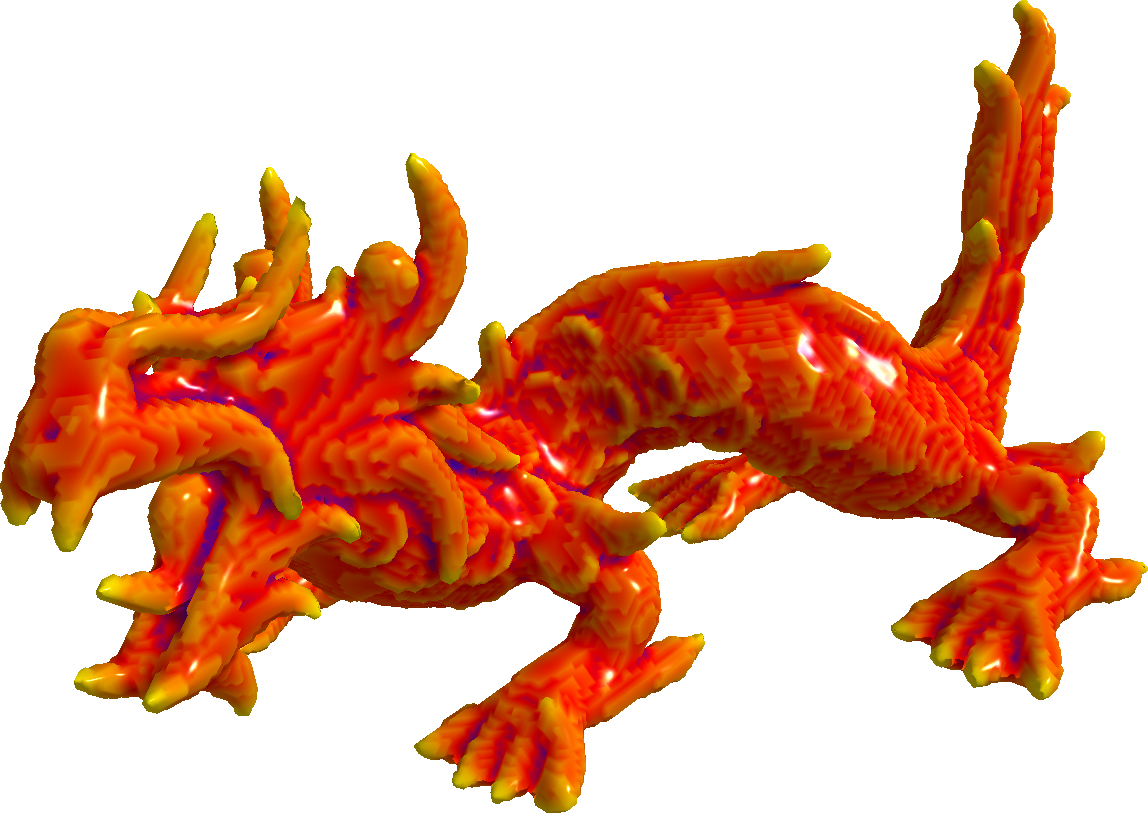
\includegraphics[height=4.0cm]{figs/xyzrgb_dragon-510_R8_mean}}
    {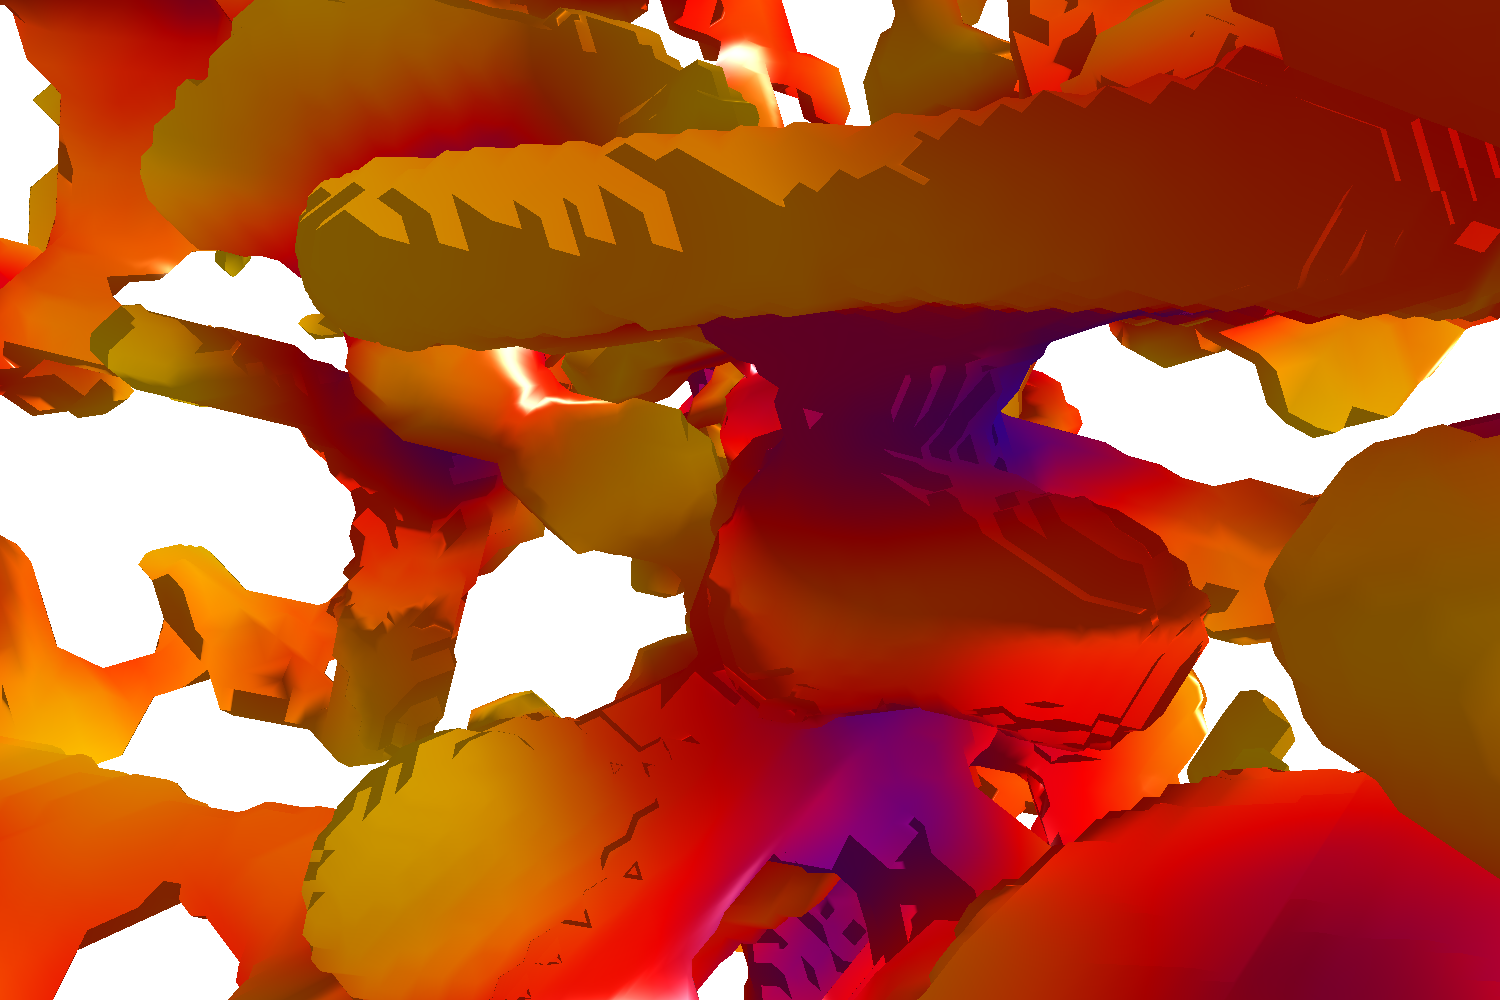
\includegraphics[height=3.5cm]{figs/snow_I08iso_233_r20_l0_m3}}
  \end{center}
  \caption{Illustration fig illustration complete (adaptative, ...) plusieurs
    objets.. + dynamique.
    Illustration of mean curvature computation of snow microstructures.
    %
    \emph{Third row:} mean curvature computed in real-time on a dynamic object.}
  \label{fig:adaptive}
\end{figure}

Figure~\ref{fig:adaptive} shows curvature computation and exploration in
real-time on large datasets: XYZ-Dragon (with digital domain of $512^3$) and
Snow microstructures ($233^3$).

\section{Conclusion and Discussion}
\label{sec:discussion}

In this article, we have propose a full data parallel framework on GPU
hardware which combines an adaptive isosurface construction from
digital data with a curvature tensor estimation at each vertex. Using
this approach, we can explore in real-time different curvature
measurements (mean, Gaussian, principal directions) with different
ball radii on potentially large dynamic dataset. Our proposal relies
on both a linear octree representation with Morton codes and an
efficient integral computation on GPU. The source code and additional
material (video, \ldots) are available on the project website
(\url{https://github.com/dcoeurjo/ICTV}).

An extension of this framework could be to implement an approximate hierarchical
algorithm. From there, we could use the dynamic refinement scheme to compute
the curvature with the hierarchical algorithm, thus massively reducing the number of probes.
We could also use trexture streaming to compute on the fly on the CPU the subdivision and
stream it to the GPU, allowing dynamic radii change with the hierarchical algorithm.
This framework could also be used for feature detection purposes
such as presented in \cite{SMI2015}. The point classification is done by computing
the curvature at different radii and comparing them. Using our framework,
this may be done in a real-time manner.
The computed curvature could finally be used to control the refinement of the
triangulation. We are for now only using the normal computation for shading
purposes but we could imagine using it along with the vertices to do a
Poisson reconstruction of the object.

%% \appendix
%% \section{Hierarchical Probing Algorithm}



%% A {\em cell} is a tuple $(k,x,y,z)$, which represents a region of the space of size $2^k \times
%% 2^k \times 2^k$, characterized by its integer coordinates $x,y,z$,
%% with $0 \le x < 2^k$, $0 \le y < 2^k$, $0 \le z < 2^k$. Cells forms an
%% octree decomposition of a cubic space. We use functions Up, Down and
%% Next to navigate between cells.


%% \begin{algorithm}
%% \KwIn{Integers $p,q,r$ \tcp*{the moment orders, with $0 \le p+q+r \le 2$}}
%% \KwIn{Integer $k$ \tcp*{$(2^k)^3$ is the size of the digital shape image}}
%% \KwIn{Mipmap $V$ \tcp*{array of $k+1$ images of sizes $(2^k)^3,  (2^{k-1})^3, \ldots,  1^3$}}
%% \KwIn{Integers $x_0,y_0,z_0$, Real $r$ \tcp*{Ball radius $r$ and center $(x_0,y_0,z_0)$}}
%% \KwOut{Real $m$ \tcp*{estimation of the $p,q,r$-moment of $X \cap B_r(x_0,y_0,z_0)$}}
%% \KwData{Cell $c :=  (k,0,0,0)$ \tcp*{Starts from biggest cell}}
%% \KwData{Integer $n := 2^k$ \tcp*{Size of each cell}}
%% \KwData{Real $d,\delta,l$ \tcp*{variables for intermediate computations}}
%% \Begin{
%%     m := 0 \;
%%     \Repeat{$c[0] = k$}{
%%       \tcp{Distance between cell and ball centers}
%%       $d := \frac{1}{2}\| 2^k(2c[1]+1,2c[2]+1,2c[3]+1) - (2x_0+1,2y_0+1,2z_0+1) \|_2$\;
%%       $\delta := \frac{\sqrt{3}}{2}2^{c[0]}$ \tcp*{half-length of cell diagonal}
%%       \If(\tcp*[f]{Is it a unit cell ?}){$c[0] = 0$}{
%%         \If(\tcp*[f]{Is cell center inside ball ?}){$d^2 \le r^2$}{
%%           $m := m + V[c] * (2^k c[1])^p * (2^k c[2])^q * (2^k c[3])^r$ \;
%%         }
%%         $c := \textsc{Next}(c)$ \tcp*{Go to next cell}
%%       } \Else{
%%         $l := \max(r-\delta,0)$\;
%%         \If(\tcp*[f]{Is cell completely inside ball ?}){$d^2 < l^2$}{
%%           $m := m + V[c] * (2^k c[1])^p * (2^k c[2])^q * (2^k c[3])^r$\;
%%           $c := \textsc{Next}(c)$ \tcp*{Go to next cell}
%%         }\ElseIf(\tcp*[f]{Is cell outside ball ?}){$d^2 > (r+\delta)^2$}{
%%           $c := \textsc{Next}(c)$ \tcp*{Go to next cell}
%%         }\lElse(\tcp*[f]{Go to a finer cell}){$c := \textsc{Down}(c)$}
%%       }
%%     }
%%     \Return{m}\;
%%   }
%%   \caption{Derecursified hierarchical algorithm for computing the
%%     $p,q,r$-moment of set $X \cap B_r(x_0,y_0,z_0)$, given a mipmap
%%     $V$ that represents the volume of a shape $X$ in each cell, and
%%     ball parameters $x_0,y_0,z_0,r$.}
%% \end{algorithm}

%% \begin{function}
%%   \caption{Up( Cell $c$ ) : Cell}
%%   \Return{Cell( $c[0]+1$, $c[1]/2$, $c[2]/2$, $c[3]/2$ )}
%% \end{function}
%% \begin{function}
%%   \caption{Down( Cell $c$ ) : Cell}
%%   \Return{Cell( $c[0]-1$, $c[1]*2$, $c[2]*2$, $c[3]*2$ )}
%% \end{function}
%% \begin{function}
%%   \caption{Next( Cell $c$ ) : Cell}
%%   \lWhile{$\mathrm{Odd}(c[1])$ and $\mathrm{Odd}(c[2])$ and $\mathrm{Odd}(c[3])$}{$c := \mathrm{Up}(c)$}
%%   \lIf{$\mathrm{Even}(c[1])$}{$c[1] := c[1]+1$}
%%   \Else{$c[1] := c[1] - 1$\;
%%     \lIf{$\mathrm{Even}(c[2])$}{$c[2] := c[2]+1$}
%%     \Else{$c[2] := c[2] - 1$\;
%%       $c[3] := c[3]+1$}
%%   }
%%   \Return{c}
%% \end{function}



\bibliographystyle{splncs03} \bibliography{ictv}
\end{document}
